%%%% kr-instructions.tex -- version 1.3 (11-Jan-2021)
\newif\ifarxiv
\arxivtrue   

\typeout{KR2026 Instructions for Authors}

% These are the instructions for authors for KR-26.

\documentclass{article}
\pdfpagewidth=8.5in
\pdfpageheight=11in

\usepackage{kr}

% Use the postscript times font!
\usepackage{amsmath}
\usepackage{amsthm}
\usepackage{amssymb}
\usepackage{times}
\usepackage{soul}
\usepackage{url}
\usepackage[hidelinks]{hyperref}
\usepackage[utf8]{inputenc}
\usepackage[small]{caption}
\usepackage{graphicx}
\usepackage{amsmath}
\usepackage{amsthm}
\usepackage{booktabs}
\usepackage{algorithm}
\usepackage{algorithmic}
\urlstyle{same}


\usepackage{subcaption}

\usepackage{tikz}

\usepackage{balance} % for balancing columns on the final page
\usepackage{multicol}
\usepackage{enumitem}
\usepackage{xspace}
\usepackage{amssymb}
\usepackage{graphicx}
\usepackage{LogicYinfeng,StrategicYinfeng}



% the following package is optional:
%\usepackage{latexsym}

% See https://www.overleaf.com/learn/latex/theorems_and_proofs
% for a nice explanation of how to define new theorems, but keep
% in mind that the amsthm package is already included in this
% template and that you must *not* alter the styling.
\newtheorem{fact}{Fact}
\newtheorem{definition}{Definition}
\newtheorem{example}{Example}
\newtheorem{proposition}{Proposition}
\newtheorem{lemma}{Lemma}
\newtheorem{theorem}{Theorem}
\newtheorem{corollary}{Corollary}
\allowdisplaybreaks


\newcommand{\appsec}[2]{%
  \ifarxiv Appendix~\ref{#1}\else Appendix, Section ``#2''\fi%
}

\newcommand{\elnote}[1] {  \footnote{\textbf{EL}: #1} }


% Following comment is from ijcai97-submit.tex:
% The preparation of these files was supported by Schlumberger Palo Alto
% Research, AT\&T Bell Laboratories, and Morgan Kaufmann Publishers.
% Shirley Jowell, of Morgan Kaufmann Publishers, and Peter F.
% Patel-Schneider, of AT\&T Bell Laboratories collaborated on their
% preparation.

% These instructions can be modified and used in other conferences as long
% as credit to the authors and supporting agencies is retained, this notice
% is not changed, and further modification or reuse is not restricted.
% Neither Shirley Jowell nor Peter F. Patel-Schneider can be listed as
% contacts for providing assistance without their prior permission.

% To use for other conferences, change references to files and the
% conference appropriate and use other authors, contacts, publishers, and
% organizations.
% Also change the deadline and address for returning papers and the length and
% page charge instructions.
% Put where the files are available in the appropriate places.
%PDF Info Is REQUIRED.
\pdfinfo{
/TemplateVersion (KR.2026.0)
}



\title{Reasoning about Welfare-Affecting Capabilities in Concurrent Games}

%\author{Anonymous Authors}

% % Single author syntax
% \iffalse % (remove the multiple-author syntax below and \iffalse ... \fi here)
% \author{%
%     Author name
%     \affiliations
%     Affiliation
%     \emails
%     email@example.com    % email
% }
% \fi
% % Multiple author syntax
\author{
Yinfeng Li$^1$\and
Emiliano Lorini$^1$\\
\affiliations
$^1$IRIT, CNRS, University of Toulouse, Toulouse, France\\
\emails
\{yinfeng.li, emiliano.lorini\}@irit.fr
}

\begin{document}

\maketitle

\begin{abstract}

We extend the languages of Coalition Logic ($\cllogic$) and Alternating-time Temporal Logic ($\atllogic$) with new modalities for welfare-affecting capabilities, capturing the benefit and harm that a coalition can bring to another coalition through its strategic choices. These languages are interpreted over concurrent games enriched with agents' preferences. On the conceptual side, we use these languages to formalize the notions of potential benefactor and danger. A potential benefactor corresponds to a coalition having the capability to confer a benefit on another coalition. Danger corresponds to a coalition having the capability to inflict harm on another coalition.  On the technical side, we present several results concerning their axiomatization, their relationships with standard $\cllogic$ and $\atllogic$, and their computational complexity.



\end{abstract}

 


 

\section{Introduction}


Understanding how agents can influence each other’s outcomes in strategic settings is a central problem in multi-agent systems. In many practical scenarios, agents or coalitions act not only to achieve their own goals but also to affect the welfare  of others, either positively or negatively. This motivates the formal study of  notions, 
such as danger and  
potential benefactor, 
that capture both the benefits and  harms that coalitions can generate through their strategic choices.

% In this paper, we focus on the  concept of  \emph{danger} and its positive counterpart
% \emph{potential boon}. 
While the general theory
of danger assumes
that dangerousness can be ascribed
not only to agents but also to
events and situations, in this paper
we focus on the dangerousness of a coalition
relative to another coalition. 
Intuitively,
a 
\emph{danger} corresponds to 
a
coalition that can inflict harm on another coalition 
by selecting a particular strategy.
In this sense the first coalition
is a danger for the second coalition.
Its
positive counterpart 
\emph{potential benefactor} corresponds to 
a coalition that can confer a benefit
on another coalition through its strategic choices. 
In this sense the first coalition
is a potential benefactor  for the second coalition.
These notions allow us to reason explicitly about the effects of coalition strategies on the welfare of others, capturing scenarios in which outcomes are not merely neutral but have qualitative significance for other agents.

Our analysis aligns with two families of philosophical theories concerning harm (and benefit) and danger.  
On the one hand, we share with the so-called \textit{non-comparative causal account of harm}~\cite{Harman2009HarmingAsCausingHarm,Bradley2012DoingAwayWithHarm} the idea that an agent or coalition harms another agent or coalition when the former brings about a bad outcome for the latter. Conversely, it is beneficial when it contributes to securing a good outcome for the latter.
The non-comparative account is traditionally contrasted with the \textit{comparative counterfactual account}, according to which an event or action is harmful to someone insofar as it makes things go worse for them, overall, than they would have been if the event or action had not occurred. 



On the other hand, we share with the  \textit{modal non-probabilistic account of danger}~\cite{Fassio2025OnDanger,Garland2003RiseOfRisk,Peschard2022PhilosophyRisk} the idea that an  agent  or coalition constitutes a danger for another agent or coalition when the former has the  potential   to  harm the latter.
The modal account is traditionally opposed to the probabilistic account, which identifies danger with risk and contrasts it with safety. Thus, while the probabilistic account conceives of danger as a high \emph{probability} of harm, the modal account focuses instead on mere \emph{possibility}. 
% \footnote{The modal account is traditionally opposed to the probabilistic account, which identifies danger with risk and contrasts it with safety. Thus, while the probabilistic account conceives of danger as a high \emph{probability} of harm, the modal account focuses instead on mere \emph{possibility}.}
In particular, we interpret \emph{potential} as the existence of a strategy available to a coalition that, if chosen, would bring harm to another coalition.\footnote{In \cite{Williamson2009ProbabilityDanger}, a counterfactual interpretation of this notion of potential or possibility is proposed. We leave for future work a comparison between our analysis and Williamson’s counterfactual theory of danger.}

The notions of good and bad are central to our analysis and, more broadly, to the theory of harm, benefit, danger, and potential benefactor. In this work, we assume that these two notions can be defined in terms of agents’ preferences: an outcome is good (resp. bad) for an agent when it is one that the agent prefers (resp. disvalues).
 
To formalize this rich conceptual framework, we build on concurrent games enriched with agents' preferences over computations, interpreted as long-term outcomes.  
We employ this class of structures to define a novel logical language based
on Alternating-time Temporal Logic ($\mathsf{ATL}$), which enables  reasoning about the  beneficial (resp.\ harmful) strategic capabilities of coalitions. 
We refer to these as the $\atlBDlogic$ language, denoting 
the extension of $\atllogic$ with \emph{welfare-affecting capabilities}.
It rests on the assumption that a coalition positively (resp.\ negatively) affects 
the welfare another coalition when the former brings benefit (resp.\ harm) to the latter through the choice of a particular strategy. 
Overall, this framework provides a rigorous basis for representing and reasoning about subtle inter-coalitional relationships, capturing the potentially beneficial or harmful influence that one coalition may exert over another.


We present  technical results concerning the axiomatizability and computational complexity of the proposed language.  
In particular, the main 
technical contributions of the paper are twofold.  

First, we provide an axiomatization of the until-free  fragment
(also called safety fragment) of the $\atlBDlogic$ language with respect to the general class of concurrent game models with \emph{regular preferences}, together with a strong notion of beneficial (resp.\ harmful) strategy. This notion is based on the idea that benefiting (resp.\ harming) a coalition means guaranteeing its best (resp.\ worst) outcome. By \emph{regular}, we mean that an agent's preference ordering 
over computations 
is stable over time, non-flat, and both well-founded and conversely well-founded. Our completeness proof relies on a novel technique based on the notion of a canonical model under formula context.

% Second, we present a variant of this axiomatization for the subclass of models in which agents' preferences are assumed to be non-flat (i.e., it is not  the case that an agent is indifferent among all outcomes). 

Second, we establish a polynomial embedding of the $\atlBDlogic$ language into standard $\atllogic$, under the regular preference assumption, as well as a polynomial embedding  of 
its coalition logic ($\cllogic$)
fragment into standard $\cllogic$. Thanks to these embeddings, we obtain tight complexity results for satisfiability checking.

Although our semantics is game-theoretic, our contribution is not merely semantic: by introducing an explicit language and an axiomatization, we can state and \emph{reason about} welfare-affecting capabilities. This is especially important when such capabilities have a temporal content (e.g., guaranteeing that a harmful situation never occurs), since standard game-theoretic representations do not, by themselves, provide a logical vocabulary to express and manipulate the temporal claims that are part of a coalition's capability.
 


The paper is organized as follows. 
Section~\ref{sec:relatedwork} discusses related work. 
Section~\ref{sec:semantics} introduces the formal semantics. 
In Section~\ref{sec:benharm}, we use this semantics to formalize the notions of beneficial and harmful strategies. 
Section~\ref{sec:languages} presents the $\atlBDlogic$ language.   
Section~\ref{sec:axiom} is devoted to the axiomatization of its
until-free fragment. 
Section~\ref{sec: tree-like model property and embedding} provides  the polynomial embeddings and
the complexity results. 
Finally, Section~\ref{conclusion} concludes the paper. Proofs are provided in a technical appendix included in the supplementary material. In particular, the supplementary material contains the proofs in \appsec{sec:app:prop_strat}{Proof of Proposition~\ref{prop:strat}}, \appsec{sec:app:completeness}{Proof of completeness for $\ourlogic$}, \appsec{sec:app:tree_like}{Proof of Theorem~\ref{theorem: tree-like property}}, and \appsec{sec:app:embedding}{Proof of Theorem~\ref{theo:embedding}}.




% Our contributions are threefold. First, we provide
% an in-depth semantic analysis of
% the notions of 
% \emph{boon} and \emph{danger}

% a formal semantics for the new modalities based on concurrent game structures with preferences, capturing both the agents’ strategic capabilities and their evaluation of outcomes. Second, we present axiomatization results, showing that the extended logics are amenable to rigorous deductive reasoning. Finally, we investigate computational properties, providing complexity results for model checking and satisfiability relative to the proposed semantics.

% By introducing the notions of boon and danger into logical reasoning about coalitions, our framework allows for a precise assessment of strategic influence in multi-agent systems. This has potential applications in automated verification, strategic planning, negotiation analysis, and the study of cooperative or adversarial behavior. Moreover, it opens avenues for integrating preference reasoning with temporal and strategic logics, contributing to a deeper understanding of multi-agent interactions and their consequences.

%%%%%%%%%%%%%%%%%%%%%%%%%%%%%%%%%%%%%%%%%%%%%%%%%%%%%%%%%%%%%%%%%%%%%%%%



 

\section{Related Work}\label{sec:relatedwork}

On the formal semantics side, our work draws on two main traditions.  
On the one hand, it builds upon the concurrent game semantics traditionally used to interpret $\mathsf{ATL}$~\cite{alur2002alternating,GorankoDrimmelenATL}, $\mathsf{CL}$~\cite{DBLP:journals/logcom/Pauly02,GorankoTARK2021}, strategy logic ($\mathsf{SL}$)~\cite{MogaveroMPV14,DBLP:conf/concur/ChatterjeeHP07}, and $\mathsf{STIT}$ (seeing-to-it-that) logic~\cite{DBLP:journals/logcom/BroersenHT06,DBLP:conf/atal/BoudouL18}.  
On the other hand, it follows the tradition of modal logics of preferences, including the pure logic of preferences and their dynamics~\cite{BenthemL07,GrossiHK22}, the interaction between preferences and epistemic states~\cite{Lorini21,Naumov2023AnEL}, and higher-order preferences~\cite{Jiang2024-JIAALO}.  
However, these works do not address the strategic or temporal dimensions of preferences.


The extension of concurrent games with preferences has recently attracted attention as a means to model agents’ rationality~\cite{DBLP:conf/ifaamas/LiLM25}, to capture the game-theoretic concept of iterated elimination of strictly dominated strategies (IESDS)~\cite{LiuEtAl2020}, and to establish connections between $\mathsf{ATL}$ strategic reasoning and correlated equilibrium~\cite{HuangRuan2017}. 
In~\cite{DBLP:conf/ifaamas/LiLM25}, a new class of models---\emph{concurrent games with preferences}---was introduced, offering a sophisticated framework for representing agents’ preferences over outcomes in concurrent games, as well as their temporal dynamics. We adopt this class of models in the present work. 
In contrast,~\cite{LiuEtAl2020} and~\cite{HuangRuan2017} focus on a simpler notion of dichotomous preference induced by an agent's goal, where the goal is expressed either directly at the model level~\cite{HuangRuan2017} or as a parameter of the modalities capturing the outcomes of the IESDS procedure~\cite{LiuEtAl2020}.
A quantitative notion of goals, based on a fuzzy interpretation, has recently been incorporated into $\mathsf{ATL}$ and $\mathsf{SL}$~\cite{jamroga2024playing,bouyer2023reasoning}, and has been used to represent agents’ utilities in the context of mechanism design~\cite{MittelmannMMP25}. 

In the present paper, we  use  concurrent games with preferences introduced in \cite{DBLP:conf/ifaamas/LiLM25}  to provide a novel logical investigation  of the notions of  beneficial  and  harmful  strategies, as well as the related concepts of  potential benefactor  and  danger, which have not previously been explored in the context of logics for multi-agent systems.
 

 

On the conceptual side, the work most closely related to ours is~\cite{BeckersChocklerHalpern2024}, which offers a causal analysis of the concept of harm based on the semantics of structural equation models. As emphasized in the introduction, there is a close connection between the notion of harm  and the notion of  danger that we investigate in this paper.
 


\section{Semantics}\label{sec:semantics}
 

In this section, we present the semantics that will later be used to define the concepts of \emph{potential benefit} and \emph{potential harm}, and to interpret the formal languages expressing these concepts. We begin with the notion of a \emph{multi-agent transition frame}. Next, we introduce \emph{concurrent game frames}, a specific class of multi-agent transition frames that satisfy a set of semantic constraints. Finally, we extend concurrent game frames by incorporating a notion of \emph{preference over computations}. 
The notion of a concurrent game with preferences is based on \cite{DBLP:conf/ifaamas/LiLM25}.




\subsection{Multi-Agent Transition Frame }

Concurrent game models can be defined from a more general class of structures, which we call \emph{multi-agent transition frames} (MATFs). An MATF is parameterized by the set of agents $\AGT = \{ 1,\ldots, n\}$, with elements denoted $a,b,\ldots$
\begin{definition}[MATF]\label{def: MATF}
    A multi agent transition frame (MATF) with respect to $\AGT$
    is a tuple 
    $\F  = (\St,  \ACT, \R)$,
    where
    \begin{itemize}
    \item $\St$ is a non-empty set of states,
    \item $\ACT$ is a set of actions,
    \item $\R: \ACT^{\AGT}\to \powerset{\St\times \St}$ assigns a transition relation on $\St$ to every action profile, where $\ACT^{\AGT}=\{\ja_{\AGT}
    \suchthat \ja_{\AGT}:
    \AGT \to \ACT\}$ is the set of action profiles.
    \end{itemize}
\end{definition}

Given an MATF as in Definition \ref{def: MATF}, we call \emph{coalitions} the subsets of $\AGT$, and we call $\AGT$ the \emph{grand coalition}. For any coalition $C$, a \emph{joint action} of $C$ is a function $\ja_{C} : C \to \ACT$, and the set of all joint actions of $C$ is denoted by $\ACT^{C}$. Note that the empty coalition has a unique joint action, $\emptyset$ (also denoted $\ja_\emptyset$), and action profiles correspond to the joint actions of the grand coalition.
Joint actions of the grand
coalition $\AGT$ are also  called \emph{action profiles}.

For any joint action $\ja_{C}$, we define
\begin{align*}
\R_{\ja_{C}} =& \big\{ (s,s') \in \St \times \St \mid{} \text{there exists } \ja_{\AGT} \in \ACT^{\AGT} \\
&\text{ such that }
\ja_{C} \subseteq \ja_{\AGT} \text{ and } (s,s') \in \R(\ja_{\AGT})\big\}.
\end{align*}
Note that in the previous
definition 
we write
$\ja_{C} \subseteq \ja_{\AGT} $
since in set theory
a function is representable as a  set of ordered pairs. We write $(s,s') \in \relAct{\ja_{C}}$ as $s \relAct{\ja_{C}} s'$, and define
\begin{align*}
\relAct{\ja_{C}}(s) = \big\{ s'\in \St \mid s \relAct{\ja_{C}} s' \big\}.
\end{align*}
It can be verified that
$\relAct{\emptyset} = \bigcup_{\ja_{\AGT} \in \ACT^{\AGT}} \relAct{\ja_{\AGT}}.$

In this paper, we treat structures and tuples as mathematical objects and use dot-notation to refer to their components or derived operations.
For example, $\M.\St$ denotes the set of all states of structure $\M$, and $t.i$ denotes the $i$-th element of tuple $t$. 

The following definition
introduces the concept
of available joint action for a coalition.
Intuitively, a joint action is available
for a coalition at a given state if the coalition 
can choose it at that state. 
\begin{definition}[Available choice]
We say that the  joint action $\ja_{C}$ is available for a coalition $C$ at a state $s$ if 
$
\relAct{\ja_{C}}(s) \neq \emptyset$. 
\end{definition}
The previous notion of available joint action  should be interpreted as what a coalition can choose at a given state:  
$
\big\{ \ja_{C} \in \ACT^{C} \mid \relAct{\ja_{C}}(s) \neq \emptyset \big\}$
is called coalition $C$'s \emph{choice set} at state $s$.




Two fundamental concepts in the semantics are those of \emph{path} and \emph{computation}, which are formally defined as follows.

\begin{definition}[Path and computation]
A \emph{path}  in a MATF $\F = (\St ,  \ACT,  \R)$ 
is a sequence $\history: \Domain \to \St$ of states, where $\Domain$ is a nonempty (possibly  infinite) initial segment of the natural numbers, such that 
\begin{align*}
\history(k) \relAct{\emptyset} \history(k+1) \quad \text{for all } k \in \Domain \text{ such that } k+1 \in \Domain.
\end{align*}
The set of all paths in $\F$ is denoted by $\Path_{\F}$. The set of all paths starting at a state $s \in \St$ is 
\begin{align*}
\Path_{\F,s} = \{ \history \in \Path_{\F} \mid \history(0) = s \}.
\end{align*}

A \emph{computation} (or \emph{full path}) in $\F$ is a path $\history \in \Path_{\F}$ such that there is no path $\history' \in \Path_{\F}$ for which $\history$ is a proper prefix. The set of all computations in $\F$ is denoted by $\Comp_{\F}$. The set of computations starting at a state $s \in \St$ is 
\begin{align*}
\Comp_{\F,s} = \{ \history \in \Comp_{\F} \mid \history(0) = s \}.
\end{align*}


A \emph{partial path} is a path that is not a computation. The set of all partial paths in $\F$ is denoted by $\PPath_{\F}$, and the set of partial paths starting at state $s \in \St$ is 
\begin{align*}
\PPath_{\F,s} = \{ \history \in \PPath_{\F} \mid \history(0) = s \}.
\end{align*}
\end{definition}


We denote the domain of a function $f$ by $\dom(f)$, the cardinality of $\dom(\history)$ by $\len(\history)$, and the restriction of $\history$ to $\{ k' \in \mathbb{N} \mid k' \le k \}$ by $\history|_k$. 
Moreover, for a finite path $\history$, we let $\END(\history)$ denote the largest element of $\dom(\history)$, and we abbreviate $\history(\END(\history))$ as $\last(\history)$.


The following fact  highlights an interesting property of partial paths, which is guaranteed by the fact that the last state of a partial path always has a successor.
\begin{fact}\label{fact:one}
$\history $ is a partial path iff 
$\history $ is finite and $\last(\history)$ is a non-terminal state, i.e., 
$\relAct{\emptyset}(\last(\history))\neq \emptyset $. 
\end{fact}


The following definition introduces the crucial notion of a \emph{joint strategy} for a coalition in a MATF. 
We define it as a \emph{total} function from partial paths to joint actions of the coalition. 
The reason for considering it as total  rather than partial is that,
in the light of Fact \ref{fact:one}, 
the last state of a  partial path always has a successor which is reachable
through a joint action
of the grand  coalition.
\begin{definition}[Joint strategy]\label{def: joint strategy}
A \emph{joint strategy} of a coalition $C$ in a MATF $\F = (\St, \ACT, \R)$
is a total  function $\js_C: \PPath_{\F} \longrightarrow  \ACT^{C}$ such that,
 for all $\history \in \dom(\js_C)$, 
$\js_C(\history)$ is available at $\last(\history)$. 
The set of all joint strategies of coalition $C$ in $\F$ is denoted by $\Js_{\F}^C$.    
\end{definition}



Given an initial state $s$ and a joint strategy for a coalition $C$, 
we can compute the set of computations generated by this strategy starting at $s$.

\begin{definition}[Generated computations]
Let $\F = (\St, \ACT, \R)$ be a MATF, $s \in \St$, 
and $\js_{C} \in \Js_{\F}^C$. 
A computation $\history$ is said to be \emph{generated} by $\js_{C}$ at $s$ if and only if:
\begin{itemize}
    \item $\history(0) = s$,
    \item 
    for all $k \in \dom(\history)$, 
    if $k+1 \in \dom(\history)$ then 
    $\history(k) \relAct{\js_C(\history|_k)} \history(k+1)$.
\end{itemize}
The set of all computations generated  by $\js_{C}$ at $s$ is denoted by $\outset_\F(s, \js_C)$.
\end{definition}


\subsection{Concurrent Game Frame }

We define concurrent game frames (CGFs)  as a subclass of MATFs. 
In particular, a CGF is a MATF which satisfies the three properties of
\emph{never-ending interaction},
\emph{independence of  choices}
and
\emph{collective choice  determinism}.


% Constraint C1 captures 
% \emph{collective choice  determinism}:
% the outcome
% of a collective choice of all agents is uniquely determined.
% Constraint C2 corresponds to the
% \emph{independence of  choices} assumption:
% if agent $1$
% can individually  choose action 
% $ \jactatm(1)$, 
% agent $2$
% can individually  choose action 
% $ \jactatm(2)$,...,
% agent $n$
% can individually  choose action 
% $ \jactatm(n)$, 
% then the agents can collectively choose joint action 
% $\jactatm$. More intuitively, this means that agents can never be deprived of choices due to the choices made by other agents.
% Constraint C3 corresponds to the 
% \emph{neverending interaction} assumption:
% every state in a CGF has
%  \emph{at least one successor},
%  where the successor of a given state
%  is a state
%  which is reachable
%  from
%  the former via
%  a collective choice
%  of all agents.

% To analyze interactions and cooperations in games, we often use the composition of strategies of disjoint coalitions, which is defined by the union of strategies with regarding strategies as sets of tuples. However, the union of strategies of disjoint coalitions is not always a joint strategy. To keep it simple, we use concurrent game frames, which is MATFs with special proerties.
\begin{definition}[CGF]\label{def: CGF}
  A MATF $\F  = (\St, \ACT, \R)$ is a concurrent game frame (CGF), if  it satisfies the following three properties:
  \begin{description}
    \item[Never-ending interaction:] 
    the relation $\R_{\emptyset}$
    over $\St$ is serial.\footnote{This means
    that $\forall s\in \St, \exists s'\in \St \text{ such that }s\R_{\emptyset} s' $. }
    \item[Independence of choices:] for all states $s \in \St$, for all coalitions $\Coalition, \Coalition'$ such that $\Coalition \cap \Coalition' = \emptyset$, and for all joint actions $\ja_{\Coalition} \in \ACT^{\Coalition}$, $\ja_{\Coalition'} \in \ACT^{\Coalition'}$, if both $\ja_{\Coalition}$ and $\ja_{\Coalition'}$ are available at $s$, then their union $\ja_{\Coalition} \cup \ja_{\Coalition'}$ is also available at $s$.

    \item[Collective choice determinism:] for every  action profile $\ja_{\AGT}$,
     the relation $\R_{\ja_{\AGT}}$
    over $\St$ is deterministic.\footnote{This means
    that $\forall s,s',s''\in \St$, if $s\R_{\ja_{\AGT}} s' $
and $s\R_{\ja_{\AGT}} s'' $ then $s'=s''$. }
  \end{description}
\end{definition}


\emph{Never-ending interaction} captures the fact that every state in a CGF has at least one successor. 
According to \emph{independence of choices}, agents can never be deprived of available actions  due to the choices made by other agents. 
Finally, \emph{collective choice  determinism} ensures
that the outcome of an available joint action of the grand coalition is uniquely determined. In other words,
once all agents have made their choices the next state is uniquely determined. 



In a CGF, computations are infinite due to the \emph{never-ending interaction} property. 
Moreover, by \emph{collective choice determinism}, the set of computations induced by a strategy of the grand coalition $\AGT$ at a given state is a singleton. 
We denote this unique computation generated by a strategy $\js_\AGT$ at state $s$ by $\out_\F(s, \js_\AGT)$. 
Finally, the \emph{independence of choices} property ensures that the merge of strategies of two disjoint coalitions yields a strategy for their union.
 



\subsection{Adding   Preferences }


We now extend a CGF with notions of preferences and regular preferences over computations, yielding the structures of a \emph{CGF with preferences} (CGFP) and a \emph{CGF with regular preferences} (CGFRP). 
Concretely, a CGF is extended by associating with each agent and each state a preference ordering over the computations starting from that state. 
Preferences satisfying stability, non-flatness, well-foundedness, and converse well-foundedness are called \emph{regular preferences}. 
This notion of preference over computations can be interpreted as a preference over long-term outcomes, since in a CGF the set of long-term outcomes available to an agent from a given state coincides with the set of computations originating from that state. 
 \begin{definition}[CGFP and CGFRP]\label{def: CGFP and CGFRP}
 A CGF with preferences (CGFP) is a tuple $\P = (\F, \preceq)$, where:
 \begin{itemize}
     \item $\F$ is a CGF, and 
     \item $\preceq: \AGT \times \St \to \powerset{\historyset_{\F}\times \historyset_{\F}}$ assigns to each agent $i \in \AGT$ and state $s \in \St$ a total preorder over $\historyset_{\F,s}$. 
 \end{itemize}
For any agent $i$, state $s$, and computations $\lambda, \lambda'$, we write
$\lambda \preceq_{i,s} \lambda'$ to denote that $(\lambda,\lambda') \in \preceq(i,s)$,
and read it as ``at state $s$, agent $i$ prefers computation $\lambda'$ at least as much as computation $\lambda$''.

 

A CGF with regular preferences
is a CGFP that satisfies the following four properties, 
for every agent $a \in \AGT$:
    \begin{align*}
       (\mathbf{SP}) \ & \forall s,s' \in \St ,
          \forall \lambda, \lambda' \in 
          \historyset_{\F,s' } 
          \text{ if } s \relAct{\emptyset }  s',
          \\ 
          &
          \text{ then }
          \big(
        \lambda'   \preceq_{a,s'}\lambda  \text{ iff }
        s \lambda'   \preceq_{a,s } s\lambda 
          \big), \\
          (\NFP)\  &\forall s\in \St, \exists \history ,\history' \in \historyset_{\F,s}\text{ such that } \history \prec_{a,s} \history' ,\\
          (\WFP)\  &\forall s\in \St, \exists \history \in \historyset_{\F,s}\text{ such that } \\
          &\forall \history' \in  \historyset_{\F,s}, \ \history \preceq_{a,s} \history' ,\\
          (\CWFP)\  &\forall s\in \St, \exists \history \in \historyset_{\F,s}\text{ such that }\\
          & \forall \history' \in \historyset_{\F,s}, \ \history' \preceq_{a,s} \history,
          \end{align*}
where, for every $\history, \history' \in\historyset_{\F,s} $, 
$\history \prec_{a,s} \history' $
abbreviates $\history \preceq_{a,s} \history' $
and
$\history'\not  \preceq_{a,s} \history $. 
% We say that the CGFP 
% $(\F,\preceq)$ has stable ($\mathbf{SP}$), non-flat ($\mathbf{NFP}$), well-founded ($\mathbf{WFP}$), or converse well-founded
% ($\mathbf{CWFP}$) preferences
% if the corresponding conditions respectively hold: for every agent $a \in \AGT$:
%           \begin{align*}
%        (\mathbf{SP}) \ & \forall s,s' \in \St ,
%           \forall \lambda, \lambda' \in 
%           \historyset_{\F,s' } 
%           \text{ if } s \relAct{\emptyset }  s',
%           \\ 
%           &
%           \text{ then }
%           \big(
%         \lambda'   \preceq_{a,s'}\lambda  \text{ iff }
%         s \lambda'   \preceq_{a,s } s\lambda 
%           \big). \\
%           (\NFP)\  &\forall s\in \St, \exists \history ,\history' \in \historyset_{\F,s}\text{ such that } \history \prec_{a,s} \history' ,\\
%           &\text{where }\lambda \prec_{i,s} \lambda'\text{ is defined as usual way}.\\
%           (\WFP)\  &\forall s\in \St, \exists \history \in \historyset_{\F,s}\text{ such that } \\
%           &\forall \in \history' \in  \historyset_{\F,s}, \ \history \preceq_{a,s} \history' .\\
%           (\CWFP)\  &\forall s\in \St, \exists \history \in \historyset_{\F,s}\text{ such that }\\
%           & \forall \in
%           \history' \in \historyset_{\F,s}, \ \history' \preceq_{a,s} \history.
%           \end{align*}
%         \begingroup\color{red}
%           A CGFP is called a CGF with regular preferences (CGFRP) if it has stable, non-flat, well-founded, and converse well-founded preferences.
%           \endgroup
\end{definition}
Property $\mathbf{SP}$ expresses stability of preferences over time. Property $\mathbf{NFP}$ ensures agents are not indifferent among all outcomes. Properties $\mathbf{WFP}$ and $\mathbf{CWFP}$

\subsection{From Frames to Models}\label{CGMRPsect}

We conclude this section by moving from
frames to models. In particular, we
assume a countably infinite  set of atomic
propositions $\AP$
denoting atomic facts and supplement 
a CGFRP  with a valuation function specifying for
every state in the CGFRP which propositions are true there.

\begin{definition}[CGMRP]\label{def: CGMRP}
  A concurrent game model with regular preferences (CGMRP) with respect to $\AGT$ and $\AP$
  is a tuple 
  $\M  = (\P, \V)$,
  where
  \begin{itemize}
  \item $\P$ is CGFRP, and 
  \item $\V: \St \to 2^\AP$ is a valuation function. 
  \end{itemize}
\end{definition}

We  illustrate 
the notion of CGMRP with the help of a concrete example. 

\begin{example}\label{ex1}
We consider a scenario involving three agents, robots $0$, $1$, and $2$, operating in a small environment composed of three rooms: a left room, a middle room, and a right room. Each of the left and right rooms contains a charging station. 
Robot~$1$ is positioned in front of the exit of the right room, guarding it to prevent entry, while robot~$2$ is stationed in front of the exit of the left room, performing the same role. 
Initially, robot~$0$ is located in the middle room (proposition $\mathit{inM}_0$). 
During the course of the game, it can move and change its position, 
entering either the right room (proposition $\mathit{inR}_0$) 
or the left room (proposition $\mathit{inL}_0$). 
The initial configuration is shown in Figure~\ref{fig:spacefigure}.

\begin{figure}[h]
    \centering
    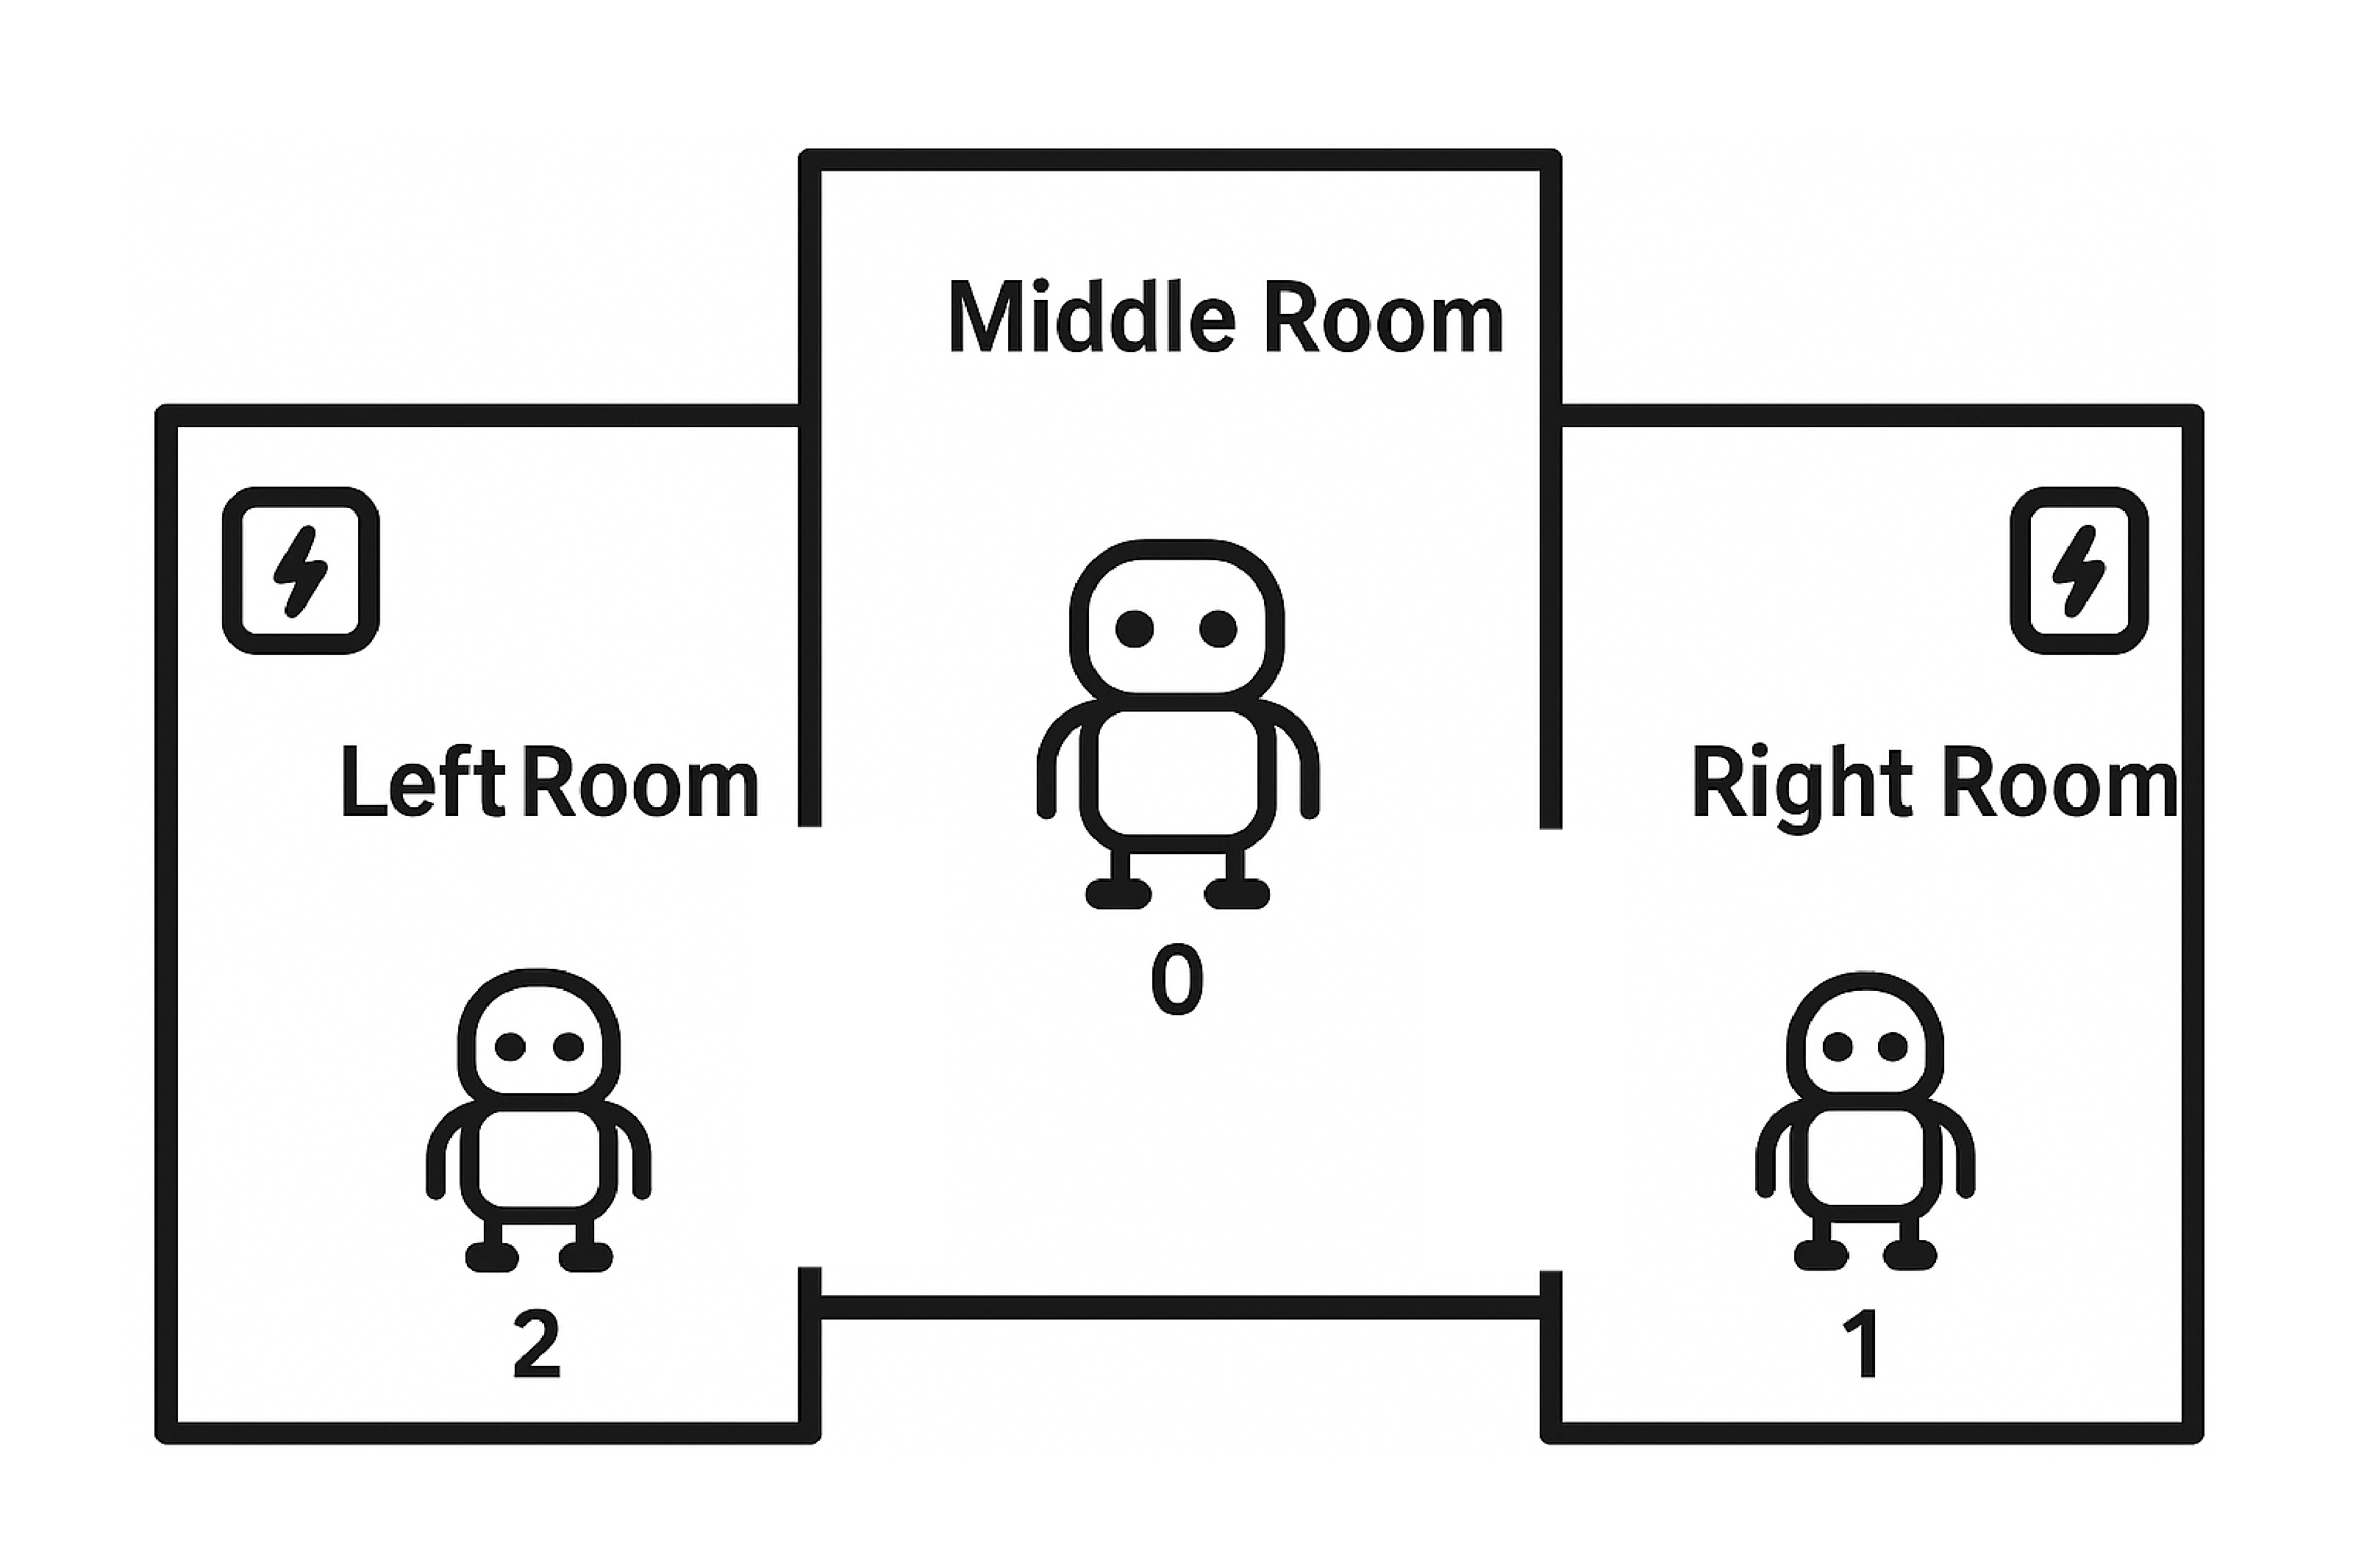
\includegraphics[width=0.55\linewidth]{ImageSpace.pdf}
    \caption{Scenario}
    \label{fig:spacefigure}
    \vspace{-1em}
\end{figure}

Robot~$0$ can move from its current room either to the right (action $\mathit{ri}$) or to the left (action $\mathit{le}$). 
Thus, to move from the middle room to the right room, it must perform the action $\mathit{ri}$; conversely, to move from the right room to the middle room, it must perform the action $\mathit{le}$, and so on. 
If robot~$0$ is already in the right (resp.\ left) room and attempts to move further right (resp.\ left), it remains in place, as it encounters a wall.

Robots~$1$ and~$2$ can either block (action~$\mathit{bl}$) or free (action~$\mathit{fr}$) 
the passage of the room they are guarding. 
Thus, robot~$1$ can block or free the passage of the right room, and robot~$2$ can do the same for the left room. 
If robot~$1$ (resp.\ robot~$2$) blocks the passage of its respective room, then robot~$0$ cannot reach the corresponding charging station when it is in the middle room, 
and cannot leave the room whose passage is blocked when it is located there.



Robot~$0$’s goal is to reach a charging station at some point in the future, while the goal of robots~$1$ and~$2$ is to prevent it from doing so. 
The CGMRP corresponding to this scenario is shown in Figure~\ref{CGMRPscenario}. 



\begin{figure}[h]
    \centering
    \captionsetup{skip=2pt}
    \captionsetup[subfigure]{skip=1pt}

    % --- Subfigure (a): TikZ diagram ---
    \begin{subfigure}[b]{0.5\textwidth}
        \centering
        \fbox{\begin{minipage}{0.95\linewidth}
        \centering
        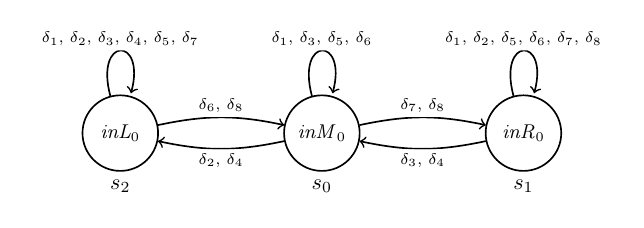
\begin{tikzpicture}[
            scale=0.8, transform shape,
            semithick,
            state/.style={circle, draw, minimum size=12mm, inner sep=0pt, font=\small},
            labelbox/.style={rounded corners=2pt, inner sep=2pt, font=\scriptsize, fill=white, draw=none}
        ]
        % --- Nodes ---
        \node[state,label=below:$s_2$] (L) at (0,0) {$\mathit{inL}_0$};
        \node[state,label=below:$s_0$] (C) at (3.2,0) {$\mathit{inM}_0$};
        \node[state,label=below:$s_1$] (R) at (6.4,0) {$\mathit{inR}_0$};

        % --- Self-loops ---
        \path[->] (C) edge[loop above]
            node[above,labelbox] {$\delta_1,\,\delta_3,\,\delta_5,\,\delta_6$} ();
        \path[->] (R) edge[loop above]
            node[above,labelbox,text width=28mm,align=center]
            {$\delta_1,\,\delta_2,\,\delta_5,\,\delta_6,\,\delta_7,\,\delta_8$} ();
        \path[->] (L) edge[loop above]
            node[above,labelbox,text width=28mm,align=center]
            {$\delta_1,\,\delta_2,\,\delta_3,\,\delta_4,\,\delta_5,\,\delta_7$} ();

        % --- Directed edges between states ---
        \draw[->,bend left=12] (C) to node[midway, above,labelbox] {$\delta_7,\,\delta_8$} (R);
        \draw[->,bend left=12] (R) to node[midway, below,labelbox] {$\delta_3,\,\delta_4$} (C);
        \draw[->,bend left=12] (C) to node[midway, below,labelbox] {$\delta_2,\,\delta_4$} (L);
        \draw[->,bend left=12] (L) to node[midway, above,labelbox] {$\delta_6,\,\delta_8$} (C);
        \end{tikzpicture}
        \end{minipage}}
        \caption{State transition diagram.}
    \end{subfigure}

    \vspace{0.35em}

    % --- Subfigure (b): Delta table ---
    \begin{subfigure}[b]{0.4\textwidth}
        \centering
        \fbox{\begin{minipage}{0.98\linewidth}\vspace{-1em}
        \[
        \begin{array}{ll}
        \delta_1 = (0{:}\mathit{le}, 1{:}\mathit{bl}, 2{:}\mathit{bl}) & \delta_5 = (0{:}\mathit{ri}, 1{:}\mathit{bl}, 2{:}\mathit{bl}) \\
        \delta_2 = (0{:}\mathit{le}, 1{:}\mathit{bl}, 2{:}\mathit{fr}) & \delta_6 = (0{:}\mathit{ri}, 1{:}\mathit{bl}, 2{:}\mathit{fr}) \\
        \delta_3 = (0{:}\mathit{le}, 1{:}\mathit{fr}, 2{:}\mathit{bl}) & \delta_7 = (0{:}\mathit{ri}, 1{:}\mathit{fr}, 2{:}\mathit{bl}) \\
        \delta_4 = (0{:}\mathit{le}, 1{:}\mathit{fr}, 2{:}\mathit{fr}) & \delta_8 = (0{:}\mathit{ri}, 1{:}\mathit{fr}, 2{:}\mathit{fr})
        \end{array}
        \]
        \end{minipage}}
        \caption{Action profiles $\delta_1$--$\delta_8$.}
    \end{subfigure}

    \vspace{0.35em}

    % --- Subfigure (c): Utility definition ---
    \begin{subfigure}[b]{0.4\textwidth}
        \centering
        \fbox{\begin{minipage}{0.55\textwidth}
          \vspace{-1em}
        \begin{align*}
      \forall s\in\{s_0,s_1,s_2\},&\,
     \forall\lambda, \lambda' \in 
      \historyset_{\F_{\mathit{rs}},s}, 
       \forall i \in \{0,1,2 \}, \\
      & \lambda \preceq_{i,s } \lambda  \text{ iff } U_0(\lambda' )  \leq U_0(\lambda)
      \text{ with}\end{align*}
        \vspace{-2em}
        \begin{align*}
        U_0(\lambda)=
        \begin{cases}
        0 & \text{if } \forall  k \geq 0, 
   \{\mathit{inR}_0,\mathit{inL}_0\}  \cap \valProp(\lambda(k)) =  
      \emptyset,\\
        1 & \text{otherwise} ;
        \end{cases}\\
        U_1(\lambda)=  U_2(\lambda)=
        \begin{cases}
        0 & \text{if } \exists   k \geq 0
        \text{ such that }\\
&      \{\mathit{inR}_0,\mathit{inL}_0\}  \cap \valProp(\lambda(k)) \neq 
      \emptyset ,\\
        1 & \text{otherwise} .
        \end{cases}
        \end{align*}
        \end{minipage}}
        \caption{Utility-induced preference structure.}
    \end{subfigure}

    \caption{CGMRP 
    $\M_{\mathit{rs}}$
    for the robots' scenario: (a) state transitions, (b) action profiles, (c) preference structure.  }
    \label{CGMRPscenario}
    \vspace{-1em}
\end{figure}


It consists of three states, $s_0$, $s_1$, and $s_2$, with $s_0$ as the initial state, and eight possible action profiles, $\delta_1, \ldots, \delta_8$. 
To make the example self-contained, we assume that each robot’s preferences over computations starting from a given state are induced by a dichotomous utility function: 
this function assigns a value of~$1$ to a computation that allows the robot to achieve its goal, and a value of~$0$ otherwise. 

\end{example}





 

 




 







\section{Beneficial  and Harmful Strategy }\label{sec:benharm}

In this section, we introduce the concepts of  beneficial  and  harmful  strategies. The intuition is straightforward: the strategy of a coalition is said to be beneficial (resp. harmful) for another coalition if the choice of that strategy by the first coalition guarantees a good (resp. bad) outcome for the second coalition. We further distinguish between \emph{strongly} and \emph{weakly} beneficial (or harmful) strategies, based on two different interpretations of what constitutes a good or bad outcome for a coalition.
A strategy is \emph{strongly beneficial} (resp.\ \emph{strongly harmful}) for a coalition if it guarantees the best (resp. worst) outcome that the agents in the coalition could obtain. Conversely, a strategy is \emph{weakly beneficial} (resp.\ \emph{weakly harmful}) for a coalition if it guarantees an outcome that is better (resp.\ worse) for the agents in the coalition than the one they could obtain if the strategy were not played.

The weak notions provide a natural baseline and allow us to relate alternative welfare-improvement criteria (in particular, strong benefit/harm implies weak benefit/harm). In the semantics of the welfare-affecting strategic capability modalities of $\lang_{\atlBDlogic}$, however, we quantify only over the \emph{strong} notions, since our axiomatization and embedding into standard $\atllogic$ rely on best/worst outcomes (whose existence is guaranteed by the regularity assumptions on preferences).




The following definition introduces the concepts
of strongly beneficial and harmful strategy.
\begin{definition}[Strongly beneficial and harmful strategy]\label{def: strong help and harm}
Let $\M = (\P, \V)$ be a CGMRP with underlying CGFRP $\P = (\F, \preceq)$. We say a strategy $\js_\Coalition$ of coalition $\Coalition$ is strongly beneficial for coalition $\GroupB\subseteq \AGT$ at the state $s$
in $\M$ 
 iff $\outset_\F(s,\js_\Coalition)\subseteq \Best_{i,s}$ for every $i\in \GroupB $, where $\Best_{i,s} = \big\{\history\in \Comp_{\F,s}\mid \forall \history'\in \Comp_{\F,s} (\history'  \preceq _{i,s} \history)  \big\}$.

 Similarly, we say a strategy $\js_\Coalition$ of coalition $\Coalition$ is strongly harmful for coalition  $\GroupH\subseteq \AGT$
at the state $s$
in $\M$
 iff $\outset_\F(s,\js_\Coalition)\subseteq \Worst_{i,s}$  for every $i\in \GroupH $, where $\Worst_{i,s} = 
 \big\{\history\in \Comp_{\F,s}\mid \forall \history'\in \Comp_{\F,s} (\history \preceq _{i,s} \history') \big\}$.
 
We denote with  $\JsSB_{\M}^C(s,\GroupB)$ and $\JsSH_{\M}^C(s,\GroupH)$
the set of strongly beneficial
strategies of coalition $\Coalition$
for coalition $\GroupB$ 
and
the set of strongly harmful 
strategies of coalition $\Coalition$
for coalition $\GroupH$ at state $s$
of the CGMRP $\M$, respectively.
\end{definition}

Let us now turn to the notion of \emph{weakly} beneficial and harmful strategies.
\begin{definition}[Weakly beneficial and harmful strategy]\label{def: weak help and harm}
Let $\M = (\P, \V)$ be a CGMRP with underlying CGFRP $\P = (\F, \preceq)$.
We say a strategy $\js_\Coalition$ of coalition $\Coalition$ is weakly beneficial for coalition $\GroupB\subseteq \AGT$ at the state $s$
in $\M$
 iff $\history' \preceq_{i,s} \history$ for all $\history\in \outset_\F(s,\js_\Coalition)$, $\history'\in \Comp_{\F,s}-\outset_\F(s,\js_\Coalition)$ and $i\in \GroupB $.

 Similarly, we say a strategy $\js_\Coalition$ of coalition $\Coalition$ is weakly harmful for coalition $\GroupH\subseteq \AGT$ at the state $s$
in $\M$ iff  $\history \preceq_{i,s} \history'$ for all $\history\in \outset_\F(s,\js_\Coalition)$, $\history'\in \Comp_{\F,s}-\outset_\F(s,\js_\Coalition)$ and $i\in \GroupH $.
 
We denote with $\JsWB_{\M}^C(s,\GroupB)$ and $\JsWH_{\M }^C(s,\GroupH)$
the set of weakly beneficial
strategies of coalition $\Coalition$
for coalition $\GroupB$ and
the set of weakly  harmful 
strategies of coalition $\Coalition$
for coalition $\GroupH$ 
at state $s$
of the CGFRP $\M$, respectively.
\end{definition}

The intuition behind Definition \ref{def: weak help and harm} is that, for a strategy to be weakly beneficial (resp. harmful) for a coalition, the outcome of the strategy should be better (resp. worse) for each member of the coalition than any outcome they could obtain if a different strategy were played.
% We add the condition 
% $
% \Comp_{\F,s} \setminus \outset_\F(s,\js_\Coalition) \neq \emptyset
% $ 
% in the definition to avoid situations in which a strategy could be considered both beneficial and harmful at the same time.\el{Is it right? }


Let us return to Example~\ref{ex1} presented in Section~\ref{CGMRPsect} in order to illustrate the preceding definitions.
\begin{example}[Cont.]\label{exa:cont1}
Consider the following strategy $\js_{\{1,2\}}$ for the coalition formed by robots~$1$ and~$2$:
\begin{align*}
 &  \js_{\{1,2\}}(\lambda)=
(1{:}\mathit{bl}, 2{:}\mathit{bl}) 
 \text{ for all }\lambda \in \PPath_{\F_{\mathit{rs}}}.
\end{align*}
This strategy corresponds to blocking the passage of  both the right and left rooms indefinitely.  
It is straightforward to verify that
$\js_{\{1,2\}} \in
\JsSH_{\M_{\mathit{rs}}}^{\{1,2\}} (s_0,\{0\})$, 
and moreover,
$\js_{\{1,2\}} \in
\JsSB_{\M_{\mathit{rs}}}^{\{1,2\}} (s_0,\{1,2\})$. 
In words, the strategy $\js_{\{1,2\}}$ of coalition~$\{1,2\}$ 
is strongly harmful for robot~$0$ at state~$s_0$, 
and strongly beneficial for the coalition made of robots~$1$ and~$2$ at the same state.

Now consider the following strategy $\js_{\{1\}}'$ for robot~$1$:
\begin{align*}
 &  \js_{\{1\}}'(\lambda)=
(1{:}\mathit{bl}) 
 \text{ for all }\lambda \in \PPath_{\F_{\mathit{rs}}}.
\end{align*}
This strategy corresponds to robot~$1$ blocking the passage of the right room indefinitely.  
It is straightforward to verify that
$\js_{\{1\}}' \in
\JsWH_{\M_{\mathit{rs}}}^{\{1\}} (s_0,\{0\})$, 
and moreover,
$\js_{\{1\}}' \notin
\JsSH_{\M_{\mathit{rs}}}^{\{1\}} (s_0,\{0\})$. 
In words, the strategy $\js_{\{1\}}'$ of robot~$1$ 
is weakly harmful for robot~$0$ at state~$s_0$, 
but not strongly harmful. 



\end{example}

The following proposition 
 highlights the connection between
 strongly beneficial/harmful
 and 
  weakly beneficial/harmful. 
The proof is given in section \ref{sec:app:prop_strat} of the supplementary material.

  \begin{proposition}\label{prop:strat}
  If 
a strategy $\js_\Coalition$ 
of a coalition $\Coalition $
is strongly beneficial (resp. harmful) for a coalition at a state, then it
is also weakly beneficial (resp. harmful).  
  \end{proposition}

 

\putaway{
To get a notion of interactive help and harm, we extend the preferences of agents from outcomes to strategies.
\begin{definition}[preferences on strategies]\label{def: preferences on strategies}
 Given a CGFP $\P = (\F, \preceq)$ and two strategies $\js_C,\js_C'$ of  coalition $C$. We say a group $\Group$ \emph{weakly prefer} $\js_C$ than $\js_C'$ at state $s$, denoted by $\js_C\geq^C_{\Group,s} \js_C'$, iff for all $i\in \Group$ and $\js_{\AGT - C}\in \Js^{\AGT - C}_\F$, we have $\out_\F(s,\js_C\cup \js_{\AGT - C})\succeq_{i,s} \out_\F(s,\js_C'\cup \js_{\AGT - C})$.
 
 As usual, we write 
  write
    $\js_C >^C_{\Group,s} \js_C'$
    if 
       $\js_C \geq^C_{\Group,s} \js_C'$
       and
          $\js_C' \not \geq ^C_{\Group,s} \js_C$, and respectively denote $\leq^C_{\Group,s}$ and $<^C_{\Group,s}$ for the reverse of $\geq^C_{\Group,s}$ and $>^C_{\Group,s}$.

 We say the preference of group $\Group$ on strategies of coalition $\Coalition$ at state $s$ is strongly non-flat ($\geq^\Coalition_{\Group,s}$ is strongly non-flat) iff for all $\js_\Coalition \in \Js^\Coalition_{\F}$ there is $\js_\Coalition' \in \Js^\Coalition_{\F}$ such that $\js_\Coalition >^C_{\Group,s} \js_\Coalition'$ or $\js_\Coalition <^C_{\Group,s} \js_\Coalition'$.
\end{definition}

The preferences on strategies are pretty similar to the notion of domination on strategies. Also, the notion of interactively beneficial and harmful strategies is similar to non-dominated strategies.
\begin{definition}[strong and interactive help and harm]\label{def: strong and interactive help and harm}
 Given a CGFP $\P = (\F, \preceq)$. We say a strategy $\js_\Coalition$ of coalition $\Coalition$ is strongly and interactively beneficial for group $\Group\subseteq \AGT$, denoted by $\js_C\help^\mathtt{si}_s\Group$, iff $\geq^\Coalition_{\Group,s}$ is strongly non-flat and there is no $\js_\Coalition'\in\Js^\Coalition_\P$ such that $\js_\Coalition'>^\Coalition_{\Group,s}\js_\Coalition$.

 Similarly, we say a strategy $\js_\Coalition$ of coalition $\Coalition$ is strongly and interactively harmful for group $\Group\subseteq \AGT$, denoted by $\js_C\harm^\mathtt{si}_s\Group$, iff $\geq^\Coalition_{\Group,s}$ is strongly non-flat and there is no $\js_\Coalition'\in\Js^\Coalition_\P$ such that $\js_\Coalition'<^\Coalition_{\Group,s}\js_\Coalition$.
 
We denote $\Js_{\F}^C\help^\si_s\Group = \{\js_\Coalition\in \Js^C_\F\mid \js_C\help^\si_s\Group\}$ and $\Js_{\F}^C\harm^\si_s\Group = \{\js_\Coalition\in \Js^C_\F\mid \js_C\harm^\si_s\Group\}$.
\end{definition}

We can drop the condition of strong non-flatness to get a weak notion of interactively beneficial and harmful strategies.
\begin{definition}[weak and interactive help and harm]\label{def: weak and interactive help and harm}
 Given a CGFP $\P = (\F, \preceq)$. We say a strategy $\js_\Coalition$ of coalition $\Coalition$ is weakly and interactively beneficial for group $\Group\subseteq \AGT$, denoted by $\js_C\help^\mathtt{wi}_s\Group$, iff there is no $\js_\Coalition'\in\Js^\Coalition_\P$ such that $\js_\Coalition'>^\Coalition_{\Group,s}\js_\Coalition$.

 Similarly, we say a strategy $\js_\Coalition$ of coalition $\Coalition$ is weakly and interactively harmful for group $\Group\subseteq \AGT$, denoted by $\js_C\harm^\mathtt{wi}_s\Group$, iff there is no $\js_\Coalition'\in\Js^\Coalition_\P$ such that $\js_\Coalition'<^\Coalition_{\Group,s}\js_\Coalition$.
 
We denote $\Js_{\F}^C\help^\wi_s\Group = \{\js_\Coalition\in \Js^C_\F\mid \js_C\help^\wi_s\Group\}$ and $\Js_{\F}^C\harm^\wi_s\Group = \{\js_\Coalition\in \Js^C_\F\mid \js_C\harm^\wi_s\Group\}$.
\end{definition}

}





\section{Language }\label{sec:languages}


In this section, we leverage the semantics presented above to interpret a novel language that extends the language of $\mathsf{ATL}$ with a new family of \emph{welfare-affecting strategic capability} modalities. These modalities allow us to reason about the strategic choices of one coalition that affect another coalition, under the assumption that the strategy of one coalition affects another insofar as the first coalition's strategic choice has either a positive or a negative effect on the well-being of the second coalition, by bringing it benefit or causing it harm.



The $\atllogic$ language with \emph{welfare-affecting capability} modalities, denoted by $\lang_{\atlBDlogic} $, is defined by the following grammar:
\begin{center}\begin{tabular}{lcl}
State formula: &$\varphi $  & $\bnf p \mid \neg\varphi \mid \varphi \wedge \varphi   \mid \atlbh{\Coalition}{\GroupB}{\GroupH}\gamma $\\
Path formula: &$\gamma $ & $\bnf \X \phi \mid 
\henceforth  \varphi 
 \mid 
 (\until{\varphi}{\psi})$
\end{tabular}\end{center}
where  $p$
ranges over $\AP$,
and $\Coalition$, $\GroupB$ and $\GroupH$ range over $\powerset{\AGT}$. 
The other Boolean connectives
and constructs 
$\vee, \rightarrow, \leftrightarrow, \top, \bot $
 are defined as abbreviations in the usual way. 
For simplicity, we sometimes write $\lang_{\atlBDlogic}$ instead of $\lang_{\atlBDlogic}(\AGT, \AP)$.

 
 % $\atlop{\Coalition: \help\GroupB,\harm \GroupH}$ is also written as $\atlbh{\Coalition}{\GroupB}{\GroupH}$ for readability.

Formulas 
$\atlbh{\Coalition}{\GroupB}{\GroupH} \nexttime \varphi$,
$\atlbh{\Coalition}{\GroupB}{\GroupH} \G \varphi$,
and 
$\atlbh{\Coalition}{\GroupB}{\GroupH} (\until{\varphi}{\psi})$
capture the notion of a \emph{welfare-affecting strategic capability} to guarantee a certain fact, where this fact is expressed by a temporal formula of $\mathsf{LTL}$ (Linear Temporal Logic). 
In particular,  
$\atlbh{\Coalition}{\GroupB}{\GroupH}
\nexttime \varphi $
has to be read 
``coalition $\Coalition$ has 
a strategy,
which is beneficial for group $\GroupB$, 
harmful to group $\GroupH$, and guarantees that
$\varphi$ is going to be true in the next state'';
$\atlbh{\Coalition}{\GroupB}{\GroupH}
 \G\varphi $
has to be read 
``coalition $\Coalition$ has 
a strategy,
which is beneficial for group $\GroupB$, 
harmful to group $\GroupH$, and guarantees that   
 $\varphi$ will always be true''; 
$\atlbh{\Coalition}{\GroupB}{\GroupH}
 (\until{\varphi}{\psi} )$
has to be read 
``coalition $\Coalition$ has 
a strategy,
which is beneficial for group $\GroupB$, 
harmful to group $\GroupH$, and guarantees that   
 $\varphi$ will be true until $\psi$ is true''.



We can now define the semantic interpretation of formulas in $\lang_{\atlBDlogic}(\AGT, \AP)$.  
As in $\mathsf{ATL}$, formulas are interpreted with respect to \emph{pointed models}. 
A pointed model is:
a pair consisting of a CGMRP and one of its states, in the case of interpreting a state formula,
or a pair consisting of a CGMRP and one of its computations, in the case of interpreting a path formula.

In Section~\ref{sec:benharm}, we introduced two notions of beneficial and harmful strategies: strong and weak.  
To interpret the welfare-affecting strategic capability modalities $\atlbh{\Coalition}{\GroupB}{\GroupH}$, we consider only the strong notion. 
Specifically, the existential quantification ranges over strongly beneficial or harmful strategies of a coalition.
This choice is motivated by our technical results: strong benefit/harm is tailored to best/worst outcomes and is the notion for which we provide an axiomatization and obtain the embedding into standard $\atllogic$ under regular preferences.

The satisfaction relation, denoted by $\models$, between formulas of $\lang_{\atlBDlogic} $ and pointed models is defined inductively as follows. 
(The cases for atomic propositions and Boolean connectives are omitted, as they are standard.)
Given  $\M = (\P, \V)$ be a CGMRP with $\P = (\St, \ACT, \R, \preceq, \dots)$ as the underlying CGFRP, $s \in \St$ a state, and $\history \in \historyset_{\F,s}$ a history: 
\begin{eqnarray*}
(\M,s)  \models 
\atlbh{\Coalition}{\GroupB}{\GroupH}\gamma 
  &\Leftrightarrow &  
  \exists \js_\Coalition \in  {\JsSB^\Coalition_\M(s,\GroupB)}\\
  &&\cap {\JsSH^\Coalition_\M(s,\GroupH)}\text{ s.t. }\\
  & &\forall \history \in \outset(s, \js_\Coalition), \big(\M, \history  \big) \models \gamma , \\
  %
  (\M,\lambda) \models \X  \varphi  
  & \Leftrightarrow  & \big( \M, \history(1) \big) \models \varphi ,\\
  %
  (\M,\lambda) \models \henceforth  \varphi  
  & \Leftrightarrow  & \forall k \in \domain(\history), \text{ if }k>0\\
&&\text{then }\big( \M, \history(k) \big) \models \varphi ,\\
%
(\M,\lambda)  \models   ( \varphi\U\psi    )
     & \Leftrightarrow  & \exists k\in \domain(\history)  \text{ s.t. } k>0,\\
     && \big(\M,\history(k) \big)  \models \psi,  \text{and }\\
   && \forall h \in \domain(\history), \text{ if }0<h<k \\
&&\text{then } \big(\M, \history(h)   \big) \models \varphi.
\end{eqnarray*}

As usual, we say that a formula $\varphi\in \lang_{\atlBDlogic} $
is valid, if $(\M,s)\models \varphi$
for every 
CGMRP $\M$
and every state $s$
in $\M$.
We say it is satisfiable if $\neg \varphi$
is not valid.


With the help of the modalities $\atlbh{\Coalition}{\GroupB}{\GroupH}$, we can elegantly represent the notions of \emph{potential benefactor} and \emph{danger}.
In particular, a coalition $\Coalition$ is said to be a  potential benefactor   for another coalition $\GroupB$, denoted $\mathsf{Benef}(\Coalition, \GroupB)$, if $\Coalition$ has a strategy that is beneficial for $\GroupB$. This can be defined as an abbreviation:
\begin{align*}
   \mathsf{Benef}(\Coalition, \GroupB) \eqdef 
   \atlbh{\Coalition}{\GroupB}{\emptyset }
   \nexttime \top .
\end{align*}
Analogously, a coalition $\Coalition$ is said to be a    danger  for another coalition $\GroupH$, denoted $\mathsf{Danger}(\Coalition, \GroupH)$, if $\Coalition$ has a strategy that is harmful for $\GroupH$. Formally:
\begin{align*}
   \mathsf{Danger}(\Coalition, \GroupH) \eqdef 
   \atlbh{\Coalition}{\emptyset}{\GroupH }
   \nexttime \top .
\end{align*}

Formulas with \emph{nested} welfare-affecting strategic modalities are useful to reason about \emph{danger-enabling} and \emph{danger-disabling} strategic choices in multi-agent settings. For instance, in the robots scenario, one can express that the coalition $\{0,1\}$ has a strategy that is strongly beneficial to robot~$0$ and guarantees that in the next state robot~$0$ becomes a danger to $\{1,2\}$, even though robot~$0$ is not a danger to $\{1,2\}$ in the current state:
\begin{align*}
&\atlbh{\{0,1\}}{\{0\}}{\emptyset}\nexttime \mathsf{Danger}(\{0\},\{1,2\})
\ \wedge\ \neg \mathsf{Danger}(\{0\},\{1,2\}).
\end{align*}
Unfolding the abbreviation for $\mathsf{Danger}$, the first conjunct is equivalent to the nested formula
$
\atlbh{\{0,1\}}{\{0\}}{\emptyset}\nexttime
\big(\atlbh{\{0\}}{\emptyset}{\{1,2\}}\nexttime \top\big)
$.
Intuitively, robot~$0$ is initially not a danger because robots~$1$ and~$2$ can coordinate to block access to their rooms; however, robot~$1$ may choose to leave its passage unguarded, allowing robot~$0$ to enter and then remain in the room indefinitely, thereby preventing robots~$1$ and~$2$ from achieving their objective.


Let us go back 
to our running example introduced in Examples 
\ref{ex1}
and 
\ref{exa:cont1}
to illustrate our language.
\begin{example}[Cont.]
We have:
\begin{align*}
  &  (\M_{\mathit{rs}}, s_0)\models
    \atlbh{\{1,2 \}}{\{1,2\}}{\{0\}}
     \G (\neg \mathit{inL}_0 \wedge \neg  \mathit{inR}_0 ). 
\end{align*}
This means that, at the initial state $s_0$ of the model $\M_{\mathit{rs}}$ corresponding to the robots' scenario, 
robots $1$ and $2$ have a strategy that is harmful to robot $0$ and beneficial to themselves, 
which prevents robot $0$ from being in the left room or the right room at some point in the future.
Consequently, we have:
\begin{align*}
  &  (\M_{\mathit{rs}}, s_0)\models
   \mathsf{Benef}(\{1,2 \}, \{1,2 \})
   \wedge 
      \mathsf{Danger}(\{1,2 \}, \{0 \}).
\end{align*}
This means that, at the initial state $s_0$, 
coalition $\{1,2\}$ is a potential benefactor for itself and a danger for robot $0$.





    
\end{example}


Observe that we give a ``strict future'' interpretation to the temporal modality $\G$: 
$\G \varphi$ is true if $\varphi$ holds at all states in the strict future along the actual computation. 
In standard $\mathsf{ATL}$, a non-strict future interpretation is used. 
Analogous temporal operators for the non-strict future, in standard $\mathsf{ATL}$ style, are definable in the language $\lang_{\atlBDlogic}$ as follows:
\begin{align*}
    \atlbh{\Coalition}{B}{H} \G^\ns \varphi &\eqdef \varphi \wedge \atlbh{\Coalition}{B}{H} \G \varphi,\\
    \atlbh{\Coalition}{B}{H} (\varphi \U^\ns \psi) &\eqdef \psi \vee (\varphi \wedge \atlbh{\Coalition}{B}{H} (\varphi \U \psi)).
\end{align*}

Furthermore, the standard $\mathsf{ATL}$ strategic capability modalities 
$\atlop{\Coalition} \nexttime \varphi$, 
$\atlop{\Coalition} \henceforth^\ns \varphi$, and 
$\atlop{\Coalition} (\varphi \U^\ns \psi)$
are definable as special cases of $\atlBDlogic$ modalities:
\begin{align*}
    \atlop{\Coalition} \nexttime \varphi &\eqdef \atlbh{\Coalition}{\emptyset}{\emptyset} \nexttime \varphi,\\
    \atlop{\Coalition} \henceforth^\ns \varphi &\eqdef \atlbh{\Coalition}{\emptyset}{\emptyset} \henceforth^\ns \varphi,\\
    \atlop{\Coalition} (\varphi \U^\ns \psi) &\eqdef \atlbh{\Coalition}{\emptyset}{\emptyset} (\varphi \U^\ns \psi).
\end{align*}

For notational convenience, we denote by $\lang_{\atllogic}$ the $\atllogic$-fragment of the language $\lang_{\atlBDlogic}$ that includes only modalities of the form $\atlbh{\Coalition}{\emptyset}{\emptyset}$.

We conclude this section by defining two additional fragments of the language $\lang_{\atlBDlogic}$. 
The following grammar defines the
until-free 
\emph{safety} fragment 
$\lang_{\atlBDlogic^{-\U}}$:
\[
\varphi  \bnf p \mid \neg\varphi \mid \varphi \wedge \varphi 
\mid \atlbh{\Coalition}{\GroupB}{\GroupH} \nexttime \varphi 
\mid \atlbh{\Coalition}{\GroupB}{\GroupH} \G \varphi,
\]
while the following grammar defines the \emph{coalition logic} fragment 
$\lang_{\clBDlogic}$:
\[
\varphi  \bnf p \mid \neg\varphi \mid \varphi \wedge \varphi 
\mid \atlbh{\Coalition}{\GroupB}{\GroupH} \nexttime \varphi,
\]
where $p$ ranges over $\AP$, and $\Coalition$, $\GroupB$, and $\GroupH$ range over $2^\AGT$.









 



\section{Axiomatization}
\label{sec:axiom}

In this section, 
we introduce a new logic
$\ourlogic$
(Logic of Welfare-Affecting Strategic Capability) 
defined relative to the  until-free fragment 
$\lang_{\atlBDlogic^{-\U}}$
and prove its its completeness. 
 

\subsection{Logic}\label{subsec: axiomatization}

The following definition introduces our logic. 
\begin{definition}[Logic $\ourlogic$]
\label{definition: axiomatic system}
$\ourlogic$ consists of the following axioms:
\begin{align*}
& 
\text{All tautologies of propositional logic} \tag{$\top$} \label{ax:taut} 
\\
&
\neg \atlbh{\Coalition}{\GroupB}{\GroupH}\nexttime \bot \tag{$\mathtt{A}\text{-}\mathtt{NAAA}$} \label{ax:NAAA}
\\
&
\atlbh{\Coalition}{\GroupB}{\GroupH}\nexttime (\phi\wedge \psi)\rightarrow  \atlbh{\Coalition}{\GroupB}{\GroupH}\nexttime \phi
\tag{$\mathtt{A}\text{-}\mathtt{MG}$} \label{ax:MG}
\\
& 
\atlbh{\Coalition}{\GroupB}{\GroupH}\nexttime \phi \rightarrow  \atlbh{\Coalition'}{\GroupB'}{\GroupH'}\nexttime\varphi  \\
&  \text{for }\Coalition\subseteq \Coalition', \GroupB\supseteq \GroupB', \GroupH\supseteq \GroupH'
\tag{$\mathtt{A}\text{-}\mathtt{MC}$} \label{ax:MC}\\
&\atlop{\Coalition: \emptyset,\emptyset}\nexttime \top \tag{$\mathtt{A}\text{-}\mathtt{NEI}$} \label{ax:Ser}
\\
& 
\big(\atlbh{\Coalition}{\GroupB}{\GroupH}\nexttime \phi \wedge \atlbh{\Coalition'}{\GroupB'}{\GroupH'}\nexttime \psi \big)\rightarrow  \\
& \atlbh{\Coalition\cup\Coalition'}{\GroupB\cup \GroupB'}{\GroupH\cup \GroupH'}\nexttime (\phi\wedge\psi) \\
&\text{for }\Coalition\cap \Coalition'=\emptyset
\tag{$\mathtt{A}\text{-}\mathtt{Sup}$} \label{ax:Sup}
\\
& 
\atlbh{\Coalition}{\GroupB}{\GroupH}\nexttime (\phi\vee \psi)\rightarrow \\
& \big(\atlbh{\Coalition}{\GroupB}{\GroupH}\nexttime \phi \vee \atlbh{\AGT}{\GroupB}{\GroupH}\nexttime \psi \big)
\tag{$\mathtt{A}\text{-}\mathtt{Cro}$} \label{ax:Cro}
\\
& 
\atlbh{\Coalition}{B}{H}\G \phi \iff \\
& \atlbh{\Coalition}{B}{H}\nexttime \big(\phi \wedge \atlbh{\Coalition}{B}{H}\G \phi \big)
\tag{$\mathtt{A}\text{-}\mathtt{FP}_\G$}\label{ax:FP_G}
\\
& 
\atlop{\emptyset}\G\big(\psi \rightarrow \atlbh{\Coalition}{B}{H}\X(\phi \wedge \psi)\big ) \rightarrow \\
& \atlop{\emptyset }\G \big(\psi \rightarrow \atlbh{\Coalition}{B}{H}\G \phi \big)
\tag{$\mathtt{A}\text{-}\mathtt{GFP}_\G$}\label{ax:GFP_G}
\\
& 
\atlbh{\Agt}{\emptyset}{\{a\}}\X\top 
\tag{$\mathtt{A}\text{-}\mathtt{WFP}$}\label{ax:WFP}
\\
& 
\atlbh{\Agt}{\{a\}}{\emptyset}\X\top
\tag{$\mathtt{A}\text{-}\mathtt{CWFP}$}\label{ax:CWFP}
\\
& 
\neg \atlbh{\Coalition}{\GroupB}{\GroupH}\nexttime \top\text{ for }\GroupB\cap \GroupH\neq \emptyset
\tag{$\mathtt{A}\text{-}\mathtt{BHC}$} \label{ax:BHC} 
\end{align*}
and the following rules of inference:
\begin{align}
& \dfrac{\;\phi, \phi \rightarrow \psi \;}
{\;\psi \;} \tag{$\mathtt{MP}$} \label{ir:MP}
\\
& \dfrac{\; \phi \iff \psi \;}{\; \atlbh{\Coalition}{\GroupB}{\GroupH}\nexttime \phi \iff \atlbh{\Coalition}{\GroupB}{\GroupH}\nexttime \psi\;} 
  \tag{$\mathtt{RE}$} \label{ir:RE}
  \\
& \dfrac{\; \phi \;}{\; \atlop{\Coalition}\G \phi \;} 
  \tag{$\mathtt{Gen}$} \label{ir:Gen}
\end{align}
\end{definition}


The names of axioms and inference rules reflect their underlying intuitions. 
Axiom \ref{ax:NAAA} is called \emph{no absurd available action}, as it expresses that a coalition's available joint action cannot ensure a logically absurd result. 
Axiom \ref{ax:MG} is called \emph{monotonicity of goals}, reflecting that capabilities are monotonic with respect to goals. 
Similarly, Axiom \ref{ax:MC} captures \emph{monotonicity of coalitions}, meaning that capabilities are monotonic with respect to coalitions. 
Axiom \ref{ax:Ser} captures the  \emph{never-ending interaction} property in Definition \ref{def: CGF}. 
Axiom \ref{ax:Sup} captures \emph{superadditivity}. 
Axiom \ref{ax:Cro} is the so-called \emph{crown} axiom: it was named this way in \cite{goranko_strategic_2013} because the effectivity function of a game has the shape of a crown. 
Axiom \ref{ax:FP_G} is the \emph{fixpoint axiom for $\G$}, capturing the fixpoint character of the operator $\G$, while Axiom \ref{ax:GFP_G} is the \emph{greatest fixpoint axiom for $\G$}, reflecting its greatest post-fixpoint nature. 
Axioms \ref{ax:WFP} and \ref{ax:CWFP} capture the \emph{well-foundedness} and \emph{converse well-foundedness} of preferences, respectively. 
Finally, Axiom \ref{ax:BHC} captures \emph{benefit-harm consistency}: a coalition cannot have a strategy that is both beneficial and harmful for the same coalition at the same time, which relates to the property that agents' preferences are non-flat. 
The inference rules are \emph{modus ponens} (\ref{ir:MP}), \emph{replacement of equivalences} (\ref{ir:RE}), and \emph{generalization} (\ref{ir:Gen}).





As usual, 
for every  $\varphi \in \lang_{\atlBDlogic^{-\U}}$,
we write $\vdash
\varphi$
to mean that $\varphi $
is derivable  in $\ourlogic$,
that is,
there is a sequence of formulas $(\varphi_1, \ldots, \varphi_m)$
such that:
\begin{itemize}
\item $\varphi_m = \varphi$, and
\item for every $1 \leq k \leq m$, either $\varphi_k$
is  an instance of one of the  axiom schema of  $\ourlogic$
or there are formulas $\varphi_{k_1}, \ldots ,\varphi_{k_t} $
such that $k_1 , \ldots, k_t < k$  and $\frac{\varphi_{k_1}, \ldots ,\varphi_{k_t} }{\varphi_{k} }$
is an instance of some inference  rule of $\ourlogic$.
\end{itemize}
We say that a finite
set of formulas $X$
is consistent if $\not \vdash
\bigwedge_{\varphi \in X}
\rightarrow \bot
$. We say a formula $\varphi$
is consistent
if the singleton set $\{\varphi\}$
is consistent. 

It is straightforward to verify that all axioms of $\ourlogic$ are valid and that all inference rules preserve validity. 
Hence, the soundness of $\ourlogic$ follows. 
For completeness, we employ a technique based on canonical models under formula contexts, which is detailed in the next section.


\subsection{Completeness }
 We are going
 to prove completeness by canonical models under formula contexts. The following definition introduces the notion of formula context. 
 % So, in the rest of this section,
 % when talking about validity
 % of a formula 
 % $\varphi \in \lang_{\clBDlogic}(\AGT , \AP )$
 % we mean validity
 % of $\varphi $
 % relative to the 
 % semantics
 % $\models$. 
\begin{definition}[Formula context]\label{def: formula context}
Given a formula $\psi $, we denote the set of all subformulas of $\psi $ by $\sub(\psi)$. Let $\sub^+(\psi ) = \{\top, \bot \}\cup \sub(\psi)\cup 
\big\{\neg \phi \mid \phi \in \sub(\psi ) \big\}$, $\cl(\psi) = sub^+(\psi)\cup \big\{\atlbh{\Coalition}{B}{H} \X\phi \suchthat  \Coalition\subseteq \AGT,B\subseteq \AGT,H\subseteq \AGT, \phi \in \sub^+(\psi ) \big\}$, and  $\cl^+(\psi) = cl (\psi)\cup \big\{\neg \phi \suchthat \phi \in \cl(\psi ) \big\}$. 
We call 
\begin{align*}
   \ecl(\psi) = \cl^+(\psi)\cup 
\big\{\bigvee_{X\in \Gamma} \bigwedge_{\chi \in X} \chi  \suchthat  \Gamma\subseteq \powerset{\cl^+(\psi)} \big\} 
\end{align*}
the $\psi$-context. 
\end{definition}


We fix a formula $\psi $ and in the rest of this section
we work  under the  $\psi $-context.  
The following definition introduces the notion of 
maximal consistent set  under a $\psi $-context.

\begin{definition}[MCS under $\psi$-context]\label{def: MCS}
Let $X \subseteq \ecl(\psi)$.
% We say $X$  is consistent iff $\not \vdash \bigwedge_{\chi \in X}\chi \rightarrow \bot$. 
  We say $X $  is a maximal  consistent
  set (MCS) under the $\psi $-context iff $X$ is consistent, 
  and for every $X' \subseteq ecl(\psi )$,  if $X\subset X'$ then $X'$ is not consistent. 
\end{definition}
% Maximal consistent sets under
% the $\psi $-context are
% called canonical pseudo states under the $\psi $-context. 
The set of all maximal consistent sets under the $\psi $-context is denoted by $\PSt^\psi $. 
The following definitions introduce the basic structure of the 
canonical model.
\begin{definition}[Canonical states]\label{def: canonical states}
  We call
$s=(X,B,H)\in \PSt^\psi\times \powerset{\AGT}\times \powerset{\AGT}$ 
a canonical state under the $\psi $-context iff $B\cap H =\emptyset$. 
We denote the set of all canonical states under the $\psi $-context by $\St^{\psi }$.
\end{definition}


We now introduce the notion of a canonical action. 
\begin{definition}[Canonical  action]
Given a formula $\psi $, we define 
\begin{align*}
 &   \LocalPower =
 \big\{\atlbh{\Coalition}{B}{H}\nexttime \chi \mid \chi \in \ecl(\psi) \text{ and }
 C,B,H\in 2^\AGT 
 \big\},\\
&\ChoiceFunction =
\big\{ \choicef: \powerset{\St^{\psi }}/\{\emptyset \}\to \St^{\psi }\mid \forall \Omega \in \powerset{\St^{\psi }}/\{\emptyset \}, \ \choicef(\Omega)  \in \Omega \big\} ,\\
& \ACT^{\psi } = \LocalPower \times \AGT \times \ChoiceFunction.
\end{align*}
$\LocalPower $ is the set of local powers, $\ChoiceFunction$ the set of choice functions, and $\ACT^{\psi }$ is the set of canonical actions.
\end{definition}

The next
definition introduces
the notions of consensus. 
\begin{definition}[Consensus]
Given an action profile $\ja : \AGT \to \ACT^{\psi }$,
we define $\Consesus(\ja) = \big\{\atlbh{\Coalition}{B}{H}\nexttime \chi \in \LocalPower\suchthat  \forall a\in \Coalition, \ \big(\ja(a) \big).1=\atlbh{\Coalition}{B}{H}\nexttime \chi \big\}$. We call  $\Consesus(\ja)$ the  agents' consensus set
relative to  $\ja$.
\end{definition}


In the next definition 
we use the notion of consensus
set to define the notion
of candidate successor. 

\begin{definition}[Candidate successor]
Given a canonical state $s$ and action profile $\ja : \AGT \to \ACT^{\psi }$,
we call a state $s'$ the candidate successors of $\ja$ at $s$, iff:
\begin{itemize}
    \item for all $\atlbh{\Coalition}{B}{H}\nexttime \chi\in \Consesus(\ja)$, if $
    \vdash \bigwedge_{\phi \in X} \phi\rightarrow \atlbh{\Coalition}{B}{H}\nexttime \chi$, then $  \vdash \bigwedge_{\chi \in s.1 } \chi \rightarrow \chi$, $B\subseteq s.2$, and $H\subseteq s.3$;
    \item for all $\chi\in \ecl(\psi)$ and $B,H\in \powerset{\AGT}$, if $ \nvdash \bigwedge_{\phi \in s.1} \phi \rightarrow \atlbh{\AGT}{B}{H}\nexttime \chi$, then $\vdash \bigwedge_{\chi \in s.1 } \chi \rightarrow \neg \chi$, $B\nsubseteq s.2$, or $H\nsubseteq s.3$.
\end{itemize}
The set of all candidate successors of $\ja$ at $s$ is denoted by $\CS(s,\ja)$.
\end{definition}
The  transition relation in the canonical model is definable through the previous notion
of candidate successor.
It can be verified that
$\CS(s,\ja)\neq \emptyset $.
This guarantees
that the transition relation
in the canonical model will satisfy
the never-ending interaction property. 
However, the set of candidate successors may be not singleton. We need some mechanism to select a unique successor from the candidate successors. To this aim, we define the following notion of election. 

\begin{definition}[Election]
Given a action profile $\ja : \AGT \to \ACT^{\psi }$, we define $\te(\ja) = 
\Big ( \big(\sum_{a\in\AGT}\ja(a).2\big)\bmod n\Big ) +1$, where $n=|\AGT|$. The agent $\te(\ja)$ is called the elected agent of
the  election relative to the action profile $\ja$.
\end{definition}

We have now all elements
to the define the notion
of canonical concurrent game model. 

\begin{definition}[Canonical CGM]\label{def: canonicalCGM}
  Given a formula $\psi $, define the canonical concurrent game model as the following structure $\CM^\psi = (\St^{\psi }, \ACT^{\psi }, \R^\psi, \V^\psi)$:
  \begin{itemize}
    \item $\St^{\psi }$ is the set of all canonical states under the  $\psi $-context;
    \item $\ACT^{\psi }$ is the set of all canonical actions under $\psi $-context;
    \item $\R^\psi $ assigns to each  action profile 
    $\delta $
    a transition relation
    $\R_\ja $ on $\St$ such that for all $s,s'\in\St^\psi$ and $\ja : \AGT \to \ACT^{\psi }$, we have $s\R_\ja s'$ iff $s' = \big(\ja(a).3 \big)\big(\CS(s,\ja) \big)$, with  $a = \te(\ja)$;
    \item $\V^\psi (p) = \{(X,B,H)\in \St^\psi \mid p\in X\}$ for each atomic proposition  $p$ in $ecl(\phi)$.
  \end{itemize} 
\end{definition}

To define the prefereces of agents in the canonical model, we need to define a utility function and the order on them
\begin{definition}[Utility function in canonical model]
  Given a canonical CGM $\CM^\psi = (\St^{\psi }, \ACT^{\psi }, \R^\psi, \preceq^\psi, \V^\psi)$, for each agent $a$ and canonical state $s$, we define a utility function as $U_{a,s}: \Comp_{\M^\psi, s} \to \mathbb{Z}\cup \{-\omega,\omega\}$ such that for any computation $\history \in \Comp_{\M^\psi, s}$: 
\[
U_{a,s}(\history) = 
\begin{cases} 
\sup\{k\in \mathbb{N}\cup \{\omega\}&\mid  \forall k'<k: a\in \history(k').2\}\\
&\text{if } a\in \history(1).2,\\
-\sup\{k\in \mathbb{N}\cup \{\omega\}&\mid  \forall k'<k: a\in \history(k').3\} \\
& \text{if } a\in \history(1).3,\\
0 & \text{otherwise.}
\end{cases}
\]
where $\sup$ is the supremum function. Note $s'.2\cap s'.3=\emptyset$ for every $s'\in \St^\psi$, so $\U_{a,s}$ is well-defined.
\end{definition}
Now we can define the canonical CGMRP
\begin{definition}[Canonical CGMRP]\label{def: canonicalmodel}
  Given a formula $\psi $, define the canonical CGMRP as the following structure $\M^\psi = (\St^{\psi }, \ACT^{\psi }, \R^\psi, \preceq^\psi, \V^\psi)$:
  \begin{itemize}
    \item $(\St^{\psi }, \ACT^{\psi }, \R^\psi, \preceq^\psi, \V^\psi)$ is the canonical CGM defined in Definition \ref{def: canonicalCGM};
    \item $\preceq^\psi $ assigns to
    each agent-state pair
    $(a,s)$ a total preorder on computations starting at $s$
    such that for all $\history,\history'\in \historyset_{\M^\psi,s}$:\\
     $\history \preceq^\psi_{a,s} \history'$ iff $U_{a,s}(\history) \geq U_{a,s}(\history')$.
  \end{itemize} 
\end{definition}

The following  lemma
guarantees that every 
consistent formula
has a witness state
in the canonical model. By the lemma, 
we have the completeness. By the previous lemma, 
we can state the following result. The proof is given in section \ref{sec:app:completeness} of the supplementary material.
\begin{lemma}\label{lem: realazation}
Let $\varphi \in \lang_{\atlBDlogic^{-\U}} $ be a consistent formula. Then,  there is a state $s\in \St^\varphi$ in the canonical model $\M^\varphi$ such that $\M^\varphi,s \models \varphi$.
\end{lemma}

\begin{theorem}[Soundness and completeness]
\label{thm:soundness and completeness}
A formula $\varphi \in \lang_{\atlBDlogic^{-\U}}$ is  valid  if and only if $\vdash \varphi$. 
\end{theorem}

\section{Tree-like  Property and Embedding}\label{sec: tree-like model property and embedding}

In this section, we show that satisfiability for the language $\lang_{\atlBDlogic}$ satisfies the tree-like model property. Based on this result, we provide polynomial embeddings of $\lang_{\atlBDlogic}$-satisfiability into $\atllogic$-satisfiability, and of $\lang_{\clBDlogic}$-satisfiability into $\cllogic$-satisfiability.
 

\subsection{Tree-like Model Property}
Let
 $\R^*$, $\R^-$ and $\R^+$
be, respectively, the reflexive and  transitive closure,
the inverse, and the transitive closure of 
$\R_\emptyset$.
\begin{definition}[Tree-like CGF]\label{def:propertiesCGF}
  Let $\F = (\St,  \ACT,   \R)$
  be a CGF.
  We say that:
  \begin{itemize}
    \item $\F$ has a unique root iff
          there is  a unique $ w_0 \in W$ (called the \emph{root}),
          such that, for every $v \in W$, $w_0 \relAct{ }^* v$;
    \item $\F$ has unique predecessors iff
          for every $v \neq w_0 $, the cardinality of $\relAct{ }^-( v)$ is at most one;
    \item $\F$ has no cycles iff $\relAct{ }^+$ is irreflexive;
    
    \item $\F$ is tree-like iff  it has a unique root,
 unique predecessors and no cycles.    
  \end{itemize}
\end{definition}
The previous definition
of tree-like CGF extends
to tree-like CGFRP
and tree-like CGMRP in a natural way.  
The tree-like model property is stated in the following lemma. Its proof is given in section \ref{sec:app:tree_like} of the supplementary material. 

     %\cite{ArxivAAMAS26} %in the supplementary material. 
     % The proof is similar to the proof of tree-like model property for $\atlratlogic$ in \cite{DBLP:conf/ifaamas/LiLM25}. 
\begin{theorem}\label{theorem: tree-like property}
  For $\varphi \in \lang_{\atlBDlogic} $,
  $\varphi$
      is satisfiable 
      iff $\varphi$
      is satisfied on a pointed tree-like CGMRP. 
\end{theorem}
\subsection{Embedding}\label{sec:embedding}


Our embeddings rely on the following translation from  $\lang_{\atlBDlogic}$ to the $\atllogic$ fragment  extended with special atomic formulas:
\begin{align*}
\mathit{tr}:
\lang_{\atlBDlogic}(\AGT, \AP ) \longrightarrow
\lang_{\atllogic}(\AGT, \AP^+ ), 
\end{align*}
with $\AP^+ =\AP\cup  \big\{ \help_i \suchthat
i \in \AGT 
\big\}\cup  \big\{ \harm_i \suchthat
i \in \AGT 
\big\}$:
\begin{align*}
  \mathit{tr}(p ) &= p,\\
\mathit{tr}(\neg \varphi  ) &= \neg \mathit{tr}( \varphi  ),\\
\mathit{tr}( \varphi \wedge
\psi ) &=   \mathit{tr}( \varphi  ) \wedge \mathit{tr}( \psi   ) ,\\
\mathit{tr}( \atlbh{\Coalition}{\GroupB}{\GroupH}
\nexttime \varphi ) &=  \atlop{\Coalition} \nexttime \big(\help \GroupB \wedge \harm \GroupH \wedge \mathit{tr}( \varphi  ) \big) ,\\
\mathit{tr}( \atlbh{\Coalition}{\GroupB}{\GroupH}
\henceforth \varphi ) &=  \atlop{\Coalition}\G\big(\help \GroupB \wedge \harm \GroupH \wedge \mathit{tr}( \varphi  ) \big) ,\\
\mathit{tr}\big( \atlbh{\Coalition}{\GroupB}{\GroupH}
(\varphi\U\psi)  \big) &=  \atlop{\Coalition} \big ((\help \GroupB \wedge \harm \GroupH \wedge \mathit{tr}(\varphi))\U\\
&\qquad\qquad(\help \GroupB \wedge \harm \GroupH \wedge \mathit{tr}(\psi))  \big).
\end{align*}
 with $\help \GroupB\eqdef \bigwedge_{i \in \GroupB} \help_i$ and $\harm \GroupH\eqdef \bigwedge_{i \in \GroupH} \harm_i$. The special atomic formula $\help_i$ is read as ``agent~$i$ is benefited,'' and $\harm_i$ as ``agent~$i$ is harmed''.  
The idea behind the above translation is to label, at the language level, beneficial (resp.\ harmful) strategies of a coalition $\Coalition$ for another coalition $\GroupB$ (resp.\ $\GroupH$) with the special constructs $\help \GroupB$ (resp.\ $\harm \GroupH$).



 


The key observation underlying the embedding for the full language $\lang_{\atlBDlogic}$ is that, in a tree-like model, whether a coalition’s strategy is beneficial or harmful for an agent depends only on whether the next state is the second element of a best (resp.\ worst) computation for that agent. 
Stability of preferences ensures that the $\help \GroupB$/$\harm \GroupH$-labeling assigned at the current state remains consistent over time.

As the following theorem shows, by using the translation $ \mathit{tr}$, satisfiability for the language $\lang_{\atlBDlogic}$ is reducible to $\atllogic$-satisfiability, and satisfiability for the fragment $\lang_{\clBDlogic}$ is reducible to $\cllogic$-satisfiability. Its proof is given in section \ref{sec:app:embedding} of the supplementary material. %\cite{ArxivAAMAS26}. %in the supplementary material.
 \begin{theorem}\label{theo:embedding}
     Let $\varphi \in \lang_{\atlBDlogic} $
     and $\psi  \in \lang_{\clBDlogic} $. 
     Then, 
     \begin{itemize}
         \item $\varphi $
     is satisfiable 
     iff $\mathit{tr}(\varphi) \wedge \bigwedge_{a\in\AGT}(\atlop{\AGT}\X\help_a\wedge\atlop{\AGT}\X\harm_a)\wedge \atlop{\emptyset }\G\big(\bigwedge_{a\in\AGT}(\atlop{\AGT}\X\help_a\wedge\atlop{\AGT}\X\harm_a \wedge \neg(\help_a\wedge\harm_a) )\big)$
     is satisfiable;
     % \elnote{
     % I think there is problem
     % in the formula of the first item. We need to move the empty-coalition modality
     % outside. Please check. 
     
     % }

     \item 
     $\psi $
     is satisfiable   
     iff $\mathit{tr}(\psi) \wedge \bigwedge_{a\in\AGT}
     \big(\atlop{\AGT}\X\help_a\wedge\atlop{\AGT}\X\harm_a\wedge\atlop{\emptyset }\X\neg(\help_a\wedge\harm_a) \big)$
     is satisfiable.
     
     \end{itemize}



 \end{theorem}

By Theorem \ref{theo:embedding}, the fact that the size of $\mathit{tr}(\varphi) $
is polynomial, and the fact that satisfiability checking
for $\atllogic$
is \Exptime-complete \cite{DrimmelenLICS}
and
satisfiability checking
for $\cllogic$
is \Pspace-complete \cite{DBLP:journals/logcom/Pauly02}, we obtain  the following tight complexity result.
  \begin{corollary}
Checking satisfiability of
 formulas in $\lang_{\atlBDlogic}$
is  \Exptime-complete.
It is \Pspace-complete 
when 
restricting to the fragment $\lang_{\clBDlogic}$. 
  \end{corollary}

%%%%%%%%%%%%%%%%


\section{Conclusion}\label{conclusion}

We have introduced a novel language based on $\mathsf{ATL}$ that enables reasoning about beneficial and harmful strategies, as well as the related notions of potential benefactor and danger. Our analysis is supported by several results concerning the axiomatizability and computational complexity of the proposed language.

The axiomatizability of the full language $\lang_{\atlBDlogic}$, including the `until' modality, remains open. We plan to address this issue in future work. We also intend to extend our analysis to a risk-based notion of danger, according to which a coalition is a danger to another coalition if it has a strategy that, if chosen, brings harm to the latter with high probability. This extension will require enriching CGMRPs with a probabilistic component.

Finally, we plan to combine the notion of danger investigated in this paper with a game-theoretic notion of rationality in order to define the concept of \emph{strong danger}: a coalition $\Coalition$ is a strong danger to another coalition $\GroupH$ if it has a \emph{rational} strategy that, if chosen, brings harm to $\GroupH$. It is called strong because it is realistic to assume that the agents in $\Coalition$ may choose the harmful strategy, provided they act rationally.

\section*{AI Declaration}
We used generative AI tools (OpenAI Codex/ChatGPT) to help identify typos and improve readability (e.g., phrasing and grammar). All scientific content, definitions, proofs, and claims were produced and verified by the authors, who take full responsibility for the paper.





\bibliographystyle{kr}
 \bibliography{bib-PHH}


\ifarxiv
\newpage 
\appendix

\allowdisplaybreaks
\section{Proof of completeness for $\clSBDlogic$}\label{sec: proof of completeness for SCA-CL}
In this section, we show the proof of completeness for $\clSBDlogic$ in details. The key step is constructing a model for any satisfiable standard conjunction, which equals to the negation of a standard disjunction. We use a method called `blueprint' to achieve it.

\subsection{Some derivabilities}\label{section: some derivabilities}
Define $\atlop{\Coalition}\G^w\phi = \phi \wedge \atlop{\Coalition}\G\phi$
\begin{theorem}
  The following are derivable in $\clSBDlogic$:
  %\tag{$\mathtt{A}\text{-}\mathtt{MC}1$} \label{ax:MC1}
  \begin{align*}  
    %No absurd rational actions
    & \dfrac{\; \phi \;}{\; \atlop{\Coalition}\G^w \phi \;} 
  \tag{$\mathtt{Gen}_{\G^w}$} \label{ir:Gen_Gw}
  \\
    & 
     \atlop{\emptyset}\G^w\big (\theta \to \atlop{\Coalition}\X(\phi \wedge \theta)\big ) 
     \to  \atlop{\emptyset }\G^w (\theta \to \atlop{\Coalition}\G \phi)  \tag{$\mathtt{th}\text{-}\mathtt{GFP}_\G$} \label{th:GFP_G}
     \\
    & 
     \atlop{\emptyset}\G^w\big (\theta \to (\phi \wedge \atlop{\Coalition}\X\theta)\big ) \to \atlop{\emptyset }\G^w (\theta \to \atlop{\Coalition}\G^w \phi)  \tag{$\mathtt{th}\text{-}\mathtt{GFP}_{\G^w}$} \label{th:GFP_Gw}
     \\
    & 
     \dfrac{\; \theta \to \atlop{\Coalition}\X(\phi \wedge \theta) \;}{\; \theta \to \atlop{\Coalition}\G \phi\;}  \tag{$\mathtt{In}_\G$} \label{ir:In_G}
  \end{align*}
  \end{theorem}  


\section{Canonical method}
\begin{definition}[formula context]\label{def: formula context}
Given an formula $\psi $, denote the set of all subformulas of $\psi $ by $sub(\psi)$. Let $sub^+(\psi ) = \{\top, \bot \}\cup sub(\psi)\cup \{\neg \phi \mid \phi \in sub(\psi )\}$, $cl(\psi) = sub^+(\psi)\cup \{\atlop{\Coalition} \phi \mid \Coalition\subseteq \AGT, \phi \in sub^+(\psi )\}$, $cl^+(\psi) = cl (\psi)\cup \{\neg \phi \mid \phi \in cl+(\psi )\}$, and $ecl(\psi) = cl^+(\psi)\cup \{\bigvee_{s\in \Gamma} \bigwedge s\mid \Gamma\subseteq \powerset{cl^+(\psi)} \}$
\end{definition}

\begin{definition}[Maximal consistent sets]\label{def: MCS}
  We say a set $s\subseteq ecl(\phi)$ of formnulas is maximal consistent sets under $\psi $-context iff $s$ is consistent and for all $s^+\subseteq ecl(\phi )$ if $s\subset s^+$ then $s^+$ is inconsistent.
\end{definition}
Maximal consistent sets under $\psi $-context is called canonical states under $\psi $-context. The set of all maximal consistent sets under $\psi $-context by $\St^\psi $.

\begin{theorem}
    For all $\Omega \subseteq \St^\psi$, there is a formula $\chi \in ecl(\phi)$ such that for all $s\subseteq \St^\psi$ we have $\chi \in s$ iff $s\in \Omega$.
\end{theorem}
In the previous theorem we call
$\chi$
the characteristic
formula
of $\Omega$. 

\newcommand{\LocalPower}{\mathtt{LP}}
\newcommand{\LP}{\mathtt{LP}}
\newcommand{\ChoiceFunction}{\mathtt{CF}}
\newcommand{\CF}{\mathtt{CF}}
\newcommand{\choicef}{\mathtt{cf}}
\begin{definition}[canonical deterministic action]
Given an formula $\phi $, define 
$$\LocalPower = \{\atlop{\Coalition}\nexttime \chi \mid \chi \text{ is a characteristic formula for some } \Omega  \subseteq \St^\psi \}$$
$$\ChoiceFunction = \{ \choicef: \powerset{\St^{\psi }}/\emptyset \to \St^{\psi }\mid \choicef(\Omega)  \in \Omega \}$$
$$\ACT^{\psi } = \LocalPower \times \AGT \times \ChoiceFunction $$
where $\LocalPower $ is the set of local powers, $\ChoiceFunction$ the set of choice functions, and $\ACT^{\psi }$ is the set of canonical deterministic actions.
\end{definition}
\newcommand{\Consesus}{\mathtt{CON}}
\newcommand{\CON}{\mathtt{CON}}
\begin{definition}[support and consesus]
For every canonical deterministic action $(\atlop{\Coalition}\nexttime \chi , a , \choicef)\in \ACT^{\psi }$, define $\Fsupport((\atlop{\Coalition}\nexttime \chi , a , \choicef)) = \atlop{\Coalition}\nexttime \chi $.
For every aciton profile $\ja : \AGT \to \ACT^{\psi }$, define $\Consesus(\ja) = \{\atlop{\Coalition}\nexttime \chi \in \LocalPower\mid (\forall a\in \Coalition )\Fsupport(\ja(a))=\atlop{\Coalition}\nexttime \chi\}$. The set $\Consesus(\ja)$ is called consesus of agents on action profile $\ja$.
\end{definition}
\begin{lemma}
For all aciton profile $\ja$, we have:
\begin{itemize}
\item $\atlop{\emptyset }\X \top \in \Consesus(\ja)$.
\item For all $\atlop{\Coalition}\X \chi , \atlop{\Coalition'}\X \chi' \in \Consesus(\ja)$  with $\atlop{\Coalition}\X \chi \neq \atlop{\Coalition'}\X \chi' $, then $\Coalition \cap \Coalition' = \emptyset $.
\end{itemize}
\end{lemma}
\begin{proof}
  The first item is obvious. For the second item, suppose that there are $\atlop{\Coalition}\X \chi , \atlop{\Coalition'}\X \chi' \in \Consesus(\ja)$  with $\atlop{\Coalition}\X \chi \neq \atlop{\Coalition'}\X \chi' $ and $\Coalition \cap \Coalition' \neq \emptyset $. Then there is an agent $a\in \Coalition \cap \Coalition'$ such that $\Fsupport(\ja(a)) = \atlop{\Coalition}\X \chi $ and $\Fsupport(\ja(a)) = \atlop{\Coalition'}\X \chi' $, which contradicts to the fact that $\atlop{\Coalition}\X \chi \neq \atlop{\Coalition'}\X \chi' $.
\end{proof}
\newcommand{\DLP}{\mathtt{DLP}}
\newcommand{\CS}{\mathtt{CS}}
\begin{definition}[deducible local power and candidate successor]
For every canonical states $s\in \St^\psi$, 
define $\DLP(s) = \{ \atlop{\Coalition}\nexttime \chi \in\LP \mid s\vdash  \atlop{\Coalition}\nexttime \chi\}$, 
which is the set of deducible local powers at $s$.

For every state $s$ and every aciton profile $\ja : \AGT \to \ACT^{\psi }$, define $\CS(s,\ja) = \{s'\in\St^\psi \mid (\forall \atlop{\Coalition}\nexttime \chi\in s\cap\Consesus(\ja))\chi\in s'\}$, which is the set of candidate successors of $\ja$ at $s$.
\end{definition}
The above definition hint that the transition relation in the canonical model is defined based on the deducible local powers and candidate successors. Note $\atlop{\emptyset }\X \top \in \CS(s,\ja)\neq \emptyset$. Then the transition relation can be defined with seriality. However, the set of candidate successors may be not singleton. We need some mechanism to select a unique successor from the candidate successors. The tricky election defined below serves this purpose.

\newcommand{\vote}{\mathtt{vote}}
\newcommand{\te}{\mathtt{te}}
\begin{definition}[voting and tricky election]
For every canonical deterministic action $(\atlop{\Coalition}\nexttime \chi , a , \choicef)\in \ACT^{\psi }$, define $\vote((\atlop{\Coalition}\nexttime \chi , a , \choicef)) = a $.

For every aciton profile $\ja : \AGT \to \ACT^{\psi }$, define $\te(\ja) = (\sum_{a\in\AGT}\vote(\ja(a)))\bmod n$, where $n=\|\AGT\|$. The agent $\te(\ja)$ is called the electee of tricky election on action profile $\ja$.
\end{definition}

\newcommand{\de}{\mathtt{de}}
\begin{definition}[decision]
For every canonical deterministic action $(\atlop{\Coalition}\nexttime \chi , a , \choicef)\in \ACT^{\psi }$, define 
$$\de((\atlop{\Coalition}\nexttime \chi , a , \choicef)) = \choicef $$
\end{definition}

\begin{definition}[canonical model]\label{def: canonicalmodel}
  Given a formula $\phi $, define the following structure $\M^\psi = $:
  \begin{itemize}
    \item $(\St^{\psi })$ is the set of all canonical states under $\psi $-context;
    \item $(\ACT^{\psi })$ is the set of all canonical deterministic actions under $\psi $-context;
    \item $\R^\psi $ assigns to every action profile a a transition relation on $\St$ such that for all $s,s'\in\St^\psi$ and $\ja : \AGT \to \ACT^{\psi }$, we have $s\R_\ja s'$ iff $s' = \de(\ja(a))(\CS(s,\ja))$, where $a = \te(\ja)$;
    \item $\V^\psi (p) = \{s\in \St^\psi \mid p\in s\}$ for all propositional variable $p$ in $ecl(\phi)$.
  \end{itemize} 
\end{definition}

\begin{lemma}[Existence lemma]
For all canonical state $s\in \St^\psi$, $\atlop{\Coalition_1}\X\chi_1,\ldots, \atlop{\Coalition_k}\X\chi_k\in \DLP(s)$ and $\atlop{\Coalition}\X \chi \in \DLP(s)$ with $\atlop{\Coalition}\X \chi \notin \DLP(s)$ with $\Coalition_i\cap \Coalition_j = \emptyset $ for all $1\leq i\neq j\leq k$ and $\Coalition_i\subseteq \Coalition $ for all $1\leq i\leq k$, there is a action profile $\ja$ and a state $s'$ such that $s\R_\ja s'$ and $\chi_i\in s'$ for all $1\leq i\leq k$ and $\neg \chi\in s'$.
\end{lemma}

\begin{theorem}[Local Realization lemma]
For every coaltition $\Coalition$, canonical state $s\in \St^\psi$, and $\Omega\subseteq \St^\psi $, we have: $s\vdash \atlop{\Coalition}\X\chi $ iff there is a joint action $\ja_C$ of $\Coalition$ such that $\js_\Coalition $ is available at $s$ and $\R_{\ja_C}(s)\subseteq \Omega$, where $\chi $ is characteristic formula of $\Omega$.
\end{theorem}
\begin{proof}
    Fix coaltition $\Coalition$, canonical state $s\in \St^\psi$,  and $\Omega\subseteq \St^\psi $. Let $\chi $ be a characteristic formula of $\Omega$. From left to right, assume $s\vdash \atlop{\Coalition}\X\chi $. Let $\ja_\Coalition: \Coalition \to \ACT^\psi$ such that $\Fsupport(\ja_\Coalition(a))=\atlop{\Coalition}\X\chi$. Then $\atlop{\Coalition}\X\chi\in\Consesus(\ja_\AGT)$ for all $\ja_\AGT:\AGT\to \ACT^\psi$ with $\ja_\Coalition \subseteq \ja_\AGT $. Note there is $\ja_\AGT:\AGT\to \ACT^\psi $ such that $\ja_\Coalition \subseteq \ja_\AGT $, $\Fsupport(\ja_\AGT (b))= \atlop{\emptyset}\X\top$ for all $b\in\AGT-\Coalition$ and $\ja_\AGT $ is available at $s$.    
    Then $\ja_\Coalition$ is available at $s$. Let $\ja_\AGT:\AGT\to \ACT^\psi$ with $\ja_\Coalition \subseteq \ja_\AGT $. Note $\atlop{\Coalition}\X\chi\in\Consesus(\ja_\AGT)$ and $s\vdash \atlop{\Coalition}\X\chi $. Then $\chi \in s'$ for all $s'\in \CS(s,\ja_\AGT )$. Then $s'\in \Omega $ for all $s'\in \R_{\ja_\Coalition }(s)$.

    From right to left, assume $s\nvdash \atlop{\Coalition}\X\chi $. Let $\ja_C$ be a joint action of $\Coalition$ such that $\js_\Coalition $ is available at $s$.    
    Let $\ja_C$ be $\ja_\AGT:\AGT\to \ACT^\psi $ such that $\ja_\Coalition \subseteq \ja_\AGT $, $\Fsupport(\ja_\AGT (b))= \atlop{\emptyset}\X\top$ for all $b \in \AGT -\Coalition $. Then $\DLP(s)\cap \Consesus(\ja_\AGT) = \DLP(s)\cap \Consesus(\ja_\Coalition)$. Note $s\nvdash \atlop{\Coalition}\X\chi $. Then $\DLP(s)\cap \Consesus(\ja_\Coalition)\cup \{\neg \atlop{\Coalition}\X\chi \}$ is consistent. We want to show $\{\phi \mid \atlop{A}\X\phi \in \DLP(s)\cap \Consesus(\ja_\Coalition)\}\cup \{\neg \chi \}$ is consistent. It suffices to show that if $\vdash \bigwedge_{\atlop{A}\X\phi \in \DLP(s)\cap \Consesus(\ja_\Coalition)}\phi \to \chi $ then $\vdash \bigwedge_{\atlop{A}\X\phi \in \DLP(s)\cap \Consesus(\ja_\Coalition)}\atlop{A}\X\phi \to \atlop{\Coalition}\X\chi $. It's clear by supperadditivity.
    Therefore, there is $s'\in \St^\psi $ such that $\{\phi \mid \atlop{A}\X\phi \in \DLP(s)\cap \Consesus(\ja_\Coalition)\}\cup \{\neg \chi \}\subseteq s'$ and $s\R_{\ja_\AGT }s'$. Note $\chi \notin s'$. Then $s'\in 
    \Omega$.
\end{proof}

\begin{theorem}[$\G$-Realization Lemma]
For $s\in \St^\psi $ and $\atlop{\Coalition}\G \phi \in ecl(\phi)$, we have $\atlop{\Coalition}\G \phi\in s$ iff there is a $\Coalition$-strategy $\js_\Coalition $ such that for all $\history \in \outset(s,\js_\Coalition)$ and all $i>0$, we have $\phi \in \history[i]$.
\end{theorem}
\begin{proof}
 Fix $s\in \St^\psi $ and $\atlop{\Coalition}\G \phi \in ecl(\phi)$. From left to right, suppose that $\atlop{\Coalition}\G \phi\in s$. By axiom \ref{ax:FP_G} and Local Realization lemma, for all $s'\in |\atlop{\Coalition}\G \phi |$, there is a joint action $\ja_{\Coalition}$ such that $\R_{\ja_{\Coalition}}(s')\subseteq |\phi \wedge \atlop{\Coalition}\G \phi |$. Let $\js_\Coalition $ be a $\Coalition$-strategy $\js_\C$ such that for all $s'\in |\atlop{\Coalition}\G \phi |$ we have $\js_\C(s)$ is a joint action $\ja_{\Coalition}$ such that $\R_{\ja_{\Coalition}}(s')\subseteq |\phi \wedge \atlop{\Coalition}\G \phi |$. Let $\history \in \outset(s,\js_\Coalition)$, by induction on $i>0$, we can show that $\phi \in \history[i]$. 

 From right to left, suppose that there is a $\Coalition$-strategy $\js_\Coalition $ such that $\phi \in \history[i]$ for all $\history \in \outset(s,\js_\Coalition)$ and all $i>0$. 
 Let $\Omega = \{s\}\cup \{\history[i]\mid \history \in \outset(s,\js_\Coalition), i>0\}$ and $\chi $ be the characteristic formula of $\Omega$. 
 Note $\R_{\js_\Coalition(s')}(s')\subseteq \Omega$ for all $s'\in \Omega $. Then $s'\vdash \atlop{\Coalition}\X (\phi \wedge \chi )$ for all $s'\in \Omega $. 
 Note $\chi \in s$. It suffices to show that $\vdash \chi \to \atlop{\Coalition}\G \phi $. 
 By \ref{ir:In_G}, 
 it suffices to show that $\vdash \chi \to \atlop{\Coalition}\X(\phi \wedge \chi)$. 
 Let $s^+$ be a maximal consistent set such that $\chi \in s^+$. Note $s^+\cap ecl(\phi )\in \St^\psi $. Then $s^+\cap ecl(\phi )\in \Omega$. 
 Therefore, $s^+\cap ecl(\phi )\vdash \atlop{\Coalition}\X (\phi \wedge \chi )$. Therefore, $\vdash \chi \to \atlop{\Coalition}\X(\phi \wedge \chi)$. Therefore, $\vdash \chi \to \atlop{\Coalition}\G \phi $ and $\atlop{\Coalition}\G \phi\in s$.
\end{proof}

\begin{theorem}[$\U$-Realization Lemma]
For $s\in \St^\psi $ and $\neg \atlop{\Coalition}(\phi \U \psi) \in ecl(\phi)$, we have $\neg \atlop{\Coalition}(\phi \U \psi)\in s$ iff there is a co-$\Coalition$-strategy $\cs_\Coalition $ such that for all $\history \in \outset(s,\cs_\Coalition)$ and $i>0$, either $\psi \notin \history[i]$ or $\phi \notin \history[j]$ for some $0< j < i$.
\end{theorem}
\begin{proof}
 Fix $s\in \St^\psi $ and$\neg \atlop{\Coalition}(\phi \U \psi) \in ecl(\phi)$. From left to right, suppose that $\neg \atlop{\Coalition}(\phi \U \psi)\in s$. By axiom \ref{ax:FP_U} and Local Realization lemma, for all $s'\in |\neg \atlop{\Coalition}(\phi \U \psi) |$, there is a co-$\Coalition$-move $cm_C$ such that $\R_{\cm_C}(s')\subseteq |\neg \psi \wedge (\neg \phi \vee \neg \atlop{\Coalition}(\phi \U \psi))|$. Let $\cs_\Coalition $ be a co-$\Coalition$-strategy $\cs_\C$ such that for all $s'\in |\neg \atlop{\Coalition}(\phi \U \psi) |$ we have $\cs_\C(s)$ is a co-$\Coalition$-move $\cm_C$ such that $\R_{\cm_C}(s')\subseteq |\neg \psi \wedge (\neg \phi \vee \neg \atlop{\Coalition}(\phi \U \psi))|$. 
 Let $\history \in \outset(s,\cs_\Coalition)$, by induction on $i>0$, we can show that either $\psi \notin \history[i]$ or $\phi \notin \history[j]$ for some $0< j < i$. \footnote{Induction is similar with the one in G-ATL semantics}
 
  From right to left, suppose that there is a co-$\Coalition$-strategy $\cs_\Coalition $ such that for all $\history \in \outset(s,\cs_\Coalition)$ and $i>0$, either $\psi \notin \history[i]$ or $\phi \notin \history[j]$ for some $0< j < i$. Let $\Omega = \{s\}\cup \{\history[i]\mid \history \in \outset(s,\cs_\Coalition), i>0\}$, $\Omega = \{s\}\cup \{\history[i]\mid \history \in \outset(s,\cs_\Coalition), i>0, \psi \in \history[i]\}$ and $\chi $ be the characteristic formula of $\Omega$. 
 Note $\R_{\cs_\Coalition(s')}(s')\subseteq \Omega$ for all $s'\in \Omega $. Then $s'\vdash \atlop{\Coalition}\X (\phi \wedge \chi )$ for all $s'\in \Omega $. 
 Note $\chi \in s$. It suffices to show that $\vdash \chi \to \atlop{\Coalition}\G \phi $. 
 By \ref{ir:In_G}, 
  
  
  , $\Theta = \{s\}\cup \{\history[i]\mid \history \in \outset(s,\cs_\Coalition), i>0, \text{ there is no }0< j < i\text{ such that }\phi \notin \history[j]\}$ and $\theta $ be the characteristic formula of $\Theta$. Then $\theta \in s$, $\psi \notin s' $ for all $s'\in \Theta $. Note for all $s'\in \Theta $, $\R_{\cs_\Coalition}(s')\subseteq \Omega $ and for all $s''\in \Omega$, either $s''\in \Theta $ or $\psi \notin s' $. Therefore, $s'\vdash \neg \atlop{\Coalition}\X \neg((\neg \psi \vee \neg \phi ))$

  ...$s'\vdash \neg \atlop{\Coalition}\X \neg(\chi \wedge (\neg \psi \vee \neg \phi ))$ for all $s'\in \Omega $. It suffices to show that $\vdash \chi \to \neg \atlop{\Coalition}(\phi \U \psi)$. By \ref{ir:In_U}, it suffices to show that $\vdash \chi \to \neg \atlop{\Coalition}\X (\psi \vee (\phi \wedge \chi))$. Let $s^+$ be a maximal consistent set such that $\chi \in s^+$. Noet $s^+\cap ecl(\phi )\in \St^\psi $. Then $s^+\cap ecl(\phi )\in \Omega$. Therefore, $s^+\cap ecl(\phi )\vdash \neg \atlop{\Coalition}\X (\psi \vee (\phi \wedge \chi ))$. Therefore, $\vdash \chi \to \neg \atlop{\Coalition}\X (\psi \vee (\phi \wedge \chi))$. Therefore, $\vdash \chi \to \neg \atlop{\Coalition}(\phi \U \psi )$ and $\neg \atlop{\Coalition}(\phi \U \psi )\in s$.
\end{proof}







\subsection{Blueprints and their realizations}
\begin{definition}[Blueprint]
A blueprint is a tuple $\bp = (\ACT_0, \
\clist,\allowbreak \Blist, \Hlist)$, where:
  \begin{itemize}
  \item $\ACT_0$ is a nonempty set of actions;
  %
  \item $\clist: \ACT^{\AGT}_0 \to \lang_{\clBDlogic}(\ATM, \AGT )$ is a consequence-list function, where $\ACT^{\AGT}_0=\{\ja: \AGT\to \ACT_0\}$, and $\clist(\ja)$ is satisfiable for all $\ja \in \JACT_0$;
  %
  \item $\Blist: \ACT^{\AGT}_0 \to \powerset{\AGT}$ is a benefit-list function;
  \item $\Hlist: \ACT^{\AGT}_0 \to \powerset{\AGT}$ is a harm-list function.
  \end{itemize}
\end{definition}
\begin{theorem}[Realization]\label{theorem: realization}
  Let $\bp = (\ACT_0, \
\clist, \Blist, \Hlist)$ be a blueprint and $\chi$ be a satisfiable conjunction of propositional literals. Then there is a pointed model $(\M,s_0)$, called a realization of $\bp$ and $\chi$, where $\M=( \F, \preceq , \V)$, $\F=( \St, \ACT, \R)$, and $\R = (\relAct{\jactatm} )_{\jactatm \in \JACT}$ such that:
  \begin{itemize}
    \item $\M,s_0\models \chi$;
    \item $(\ACT_0\times \Z)\subseteq \ACT$;
    \item for all $\js_\AGT\in \Js_{M}^\AGT$ and $\ja: \AGT\to \ACT_0$, if for all $a\in \AGT $ there is $z\in \Z$ such that $\js(s_0)(a)=(\ja(a),z)$, then $(\M,\out_{\M}(s_0,\js_\AGT)(1))\models \clist(\ja)$;
    \item for all $\js_\AGT\in \Js_{M}^\AGT$ and $\ja: \AGT\to \ACT_0$, if for all $a\in \AGT $ there is $z\in \Z$ such that $\js(s_0)(a)=(\ja(a),z)$, then for all $i\in \AGT$, $\out_{\M}(s_0,\js_\AGT)\in \Best_{i,s_0}$ iff $i\in \Blist(\ja)$, and $\out_{\M}(s_0,\js_\AGT)\in \Worst_{i,s_0}$ iff $i\in \Hlist(\ja)$.
  \end{itemize}
\end{theorem}
\begin{proof}  
  For all $\ja\in\ACT^{\AGT}_0$, let $(\M^{\ja }, s^{\ja })$ be a pointed model satisfies $\clist(\ja )$, where $\M=(\St^{\ja }, \ACT^{\ja }, \R^{\ja}, \preceq^{\ja }, \V^\ja)$, their domains are pairwise disjoint, and their set of actions are pairwise disjoint and disjoint with $\ACT_0$. Let $s_0$ be three states not in any of these models. 

  Before constructing the model, we first define the pseudo-utility function $\PU: \{\ja: \AGT\to (\ACT_0\times \Z)\}\to \Z$ satisfying for all $\ja: \AGT\to (\ACT_0\times \Z)$:
  $$\PU(\ja)=\sum_{a\in \AGT}\mathit{second}(\ja(a))$$
  where $\mathit{second}(\ja(a))$ is the second element of the pair $\ja(a)$ for every $a\in \AGT$.
  
  Define the CGMP $\M=(\St, \ACT, \R, \preceq, \V)$ as the following:
  \begin{itemize}
    \item $\St=\{s_0\}\cup \bigcup_{\ja\in\ACT^{\AGT}_0}(\St^{\ja }\times \Z)$;
    \item $\ACT=(\ACT_0\times \Z)\cup \bigcup_{\ja\in\ACT^{\AGT}_0}\ACT^{\ja }$;
    \item for all $s,s'\in \St$ and $\ja: \AGT\to \ACT $: $s\R_\ja s'$ iff one of the following condition is satisfied:
    \begin{itemize}
        \item there is $\sigma\in\ACT^{\AGT}_0$, $z\in \Z$ and $u,v\in St^{\sigma}$ such that $s=(u,z)$, $s'=(v,z)$, $\ja: \AGT\to \ACT^{\sigma }$ and $u\R^{\sigma}_\ja v'$;
        \item $s=s_0$ $\ja: \AGT\to (\ACT_0\times \Z)$, there is $\sigma:\AGT \to \ACT_0$ such that $\mathit{first}(\ja(a))=\sigma(a)$ for all $a\in \AGT$ and $s'=(s^\sigma, \PU(\ja))$, where $\mathit{first}(\ja(a))$ is the first element of the pair $\ja(a)$ for every $a\in \AGT$;
    \end{itemize}
    \item for all $s \in \St$:
    $$\Va{s}=$$
    $$\begin{cases}
      \valProp^{\ja }(u)&\text{ if there is }\ja\in\ACT^{\AGT}_0 \\
      &\text{ and }z\in \Z \text{ such that }s=(u,z),\\
      \{p\in \AP \mid p \text{ is a conjunct of }\chi \}&\text{ if }s=s_0\\
    \end{cases}$$
    \item for all $a\in\AGT$ and $s \in \St$:
    $$\preceq_{a,s}=\begin{cases}
        \preceq^{\ja }_{a,s}&\text{ if }s\in \St^{\ja } \text{ for some }\ja\in\ACT^{\AGT}_0\\
        \preceq^0_a&\text{ if }s=s_0
    \end{cases}$$
    where $\preceq^0_a=\{(\history,\history')\in \historyset_{\M,s_0}\times \historyset_{\M,s_0} \mid \mathit{U}_{a}(\history)\leq \mathit{U}_{a}(\history')\}$, $\mathit{U}:\historyset_{\M,s_0}\to \Z$ is the utility function of $a$, such that for all $\history\in \historyset_{\M,s_0}$:
    \begin{itemize}
        \item if there is $\ja: \AGT \to (\ACT_0\times \Z)$ and $\sigma \in \ACT_0^{\AGT}$ such that $\mathit{first}(\ja(a))=\sigma(a)$, $a\notin \Blist(\sigma)$, $s_0\R_\ja\history(1)$ and $\PU(\ja)>0$, then $\mathit{U}_{a}(\history)=\PU(\ja)$;
        \item if there is $\ja: \AGT \to (\ACT_0\times \Z)$ and $\sigma \in \ACT_0^{\AGT}$ such that $\mathit{first}(\ja(a))=\sigma(a)$, $a\notin \Hlist(\sigma)$, $s_0\R_\ja\history(1)$ and $\PU(\ja)<0$, then  $\mathit{U}_{a}(\history)=\PU(\ja)$;
        \item otherwise $\mathit{U}_{a}(\history)=0$.
    \end{itemize}
  \end{itemize}

  It is clear that $\M,s_0\models \chi$ and $\ACT_0\subseteq \ACT$.
  
  Let $\js\in \Js_{M}^\AGT$ and $\ja: \AGT \to \ACT_0$ such that $\js(a)(s_0)=\ja(a)$ for all $a\in \AGT$. We want to show $M,\out_{M}(s_0,\js)(1)\models \clist(\ja)$. Note $\rel_\ja(s_0)=\{s^\ja\}$. Then $\out_{M}(s_0,\js)(1)=s^\ja$. Therefore, $$M,\out_{M}(s_0,\js)(1)\models \clist(\ja).$$

  Let $\js_\AGT\in \Js_{M}^\AGT$ and $\ja: \AGT\to \ACT_0$ such that $a\in \AGT $ there is $z\in \Z$ such that $\js(s_0)(a)=(\ja(a),z)$. We want to show for all $i\in \AGT$, $\out_{\M}(s_0,\js_\AGT)\in \Best_{i,s_0}$ iff $i\in \Blist(\ja)$, and $\out_{\M}(s_0,\js_\AGT)\in \Worst_{i,s_0}$ iff $i\in \Hlist(\ja)$. Let $i\in \AGT$. We only show that $\out_{\M}(s_0,\js_\AGT)\in \Best_{i,s_0}$ iff $i\in \Blist(\ja)$ here. The proof for $\out_{\M}(s_0,\js_\AGT)\in \Worst_{i,s_0}$ iff $i\in \Hlist(\ja)$ is similar. 
  
  From left to right, assume $\out_{\M}(s_0,\js_\AGT)\in \Best_{i,s_0}$. Then there is no $\history\in \historyset_{\M,s_0}$ such that $\mathit{U}_{i}(\history)>\mathit{U}_{i}(\out_{\M}(s_0,\js_\AGT))$. Note for all $k\in \N$ there is always some $\sigma: \AGT \to (\ACT_0\times \Z)$ such that $\mathit{first}(\sigma(i))=\delta(i)$,, $s_0\R_\ja\history(1)$ and $\PU(\sigma)>0$. If $i\notin \Blist $ then there is always some $\history\in \historyset_{\M,s_0}$ such that $\mathit{U}_{i}(\history)>\mathit{U}_{i}(\out_{\M}(s_0,\js_\AGT))$. Therefore, $i\in \Blist(\ja)$.

  From right to left, assume $i\in \Blist(\ja)$. Then $\mathit{U}_{i}(\history)\leq 0$ for all $\history\in \historyset_{\M,s_0}$. Note $\mathit{U}_{i}(\history)=0$ for all $\history\in \outset_{\M}(s_0,\js_\AGT)$. Therefore, $\out_{\M}(s_0,\js_\AGT)\in \Best_{i,s_0}$.
\end{proof}

\subsection{The proof of downward validity for $\clSBDlogic$}\label{subsec: the proof of downward validity}
Now we prove the downward validity lemma (Lemma \ref{lemma: downward validity}).
\begin{proof}
  We prove its contrapositive. Assume validity-reduction-condition is not met. Then it meets satisfiability-reduction-condition, that is:   
  $\neg \chi $ is satisfiable and for all $X\subseteq \NI$ and $Y \subseteq \PI $, if
\begin{itemize}
  \item $X$ is neat;
  \item $\bigcup_{\nindex\in X} \Coalition_\nindex \subseteq \Coalition_\pindex$, $\bigcup_{\nindex\in X} \GroupB_\nindex \supseteq \GroupB_\pindex$ and $\bigcup_{\nindex\in X} \GroupH_\nindex \supseteq \GroupH_\pindex$ for all $\pindex \in \PI$;
  \item and there is at most one $\pindex\in \PI$ such that $\Coalition_\pindex \neq \AGT$;
  \end{itemize}
  then $\bigwedge_{\nindex\in X} \psi_\nindex \wedge \bigwedge_{\pindex\in Y}\neg \psi_{\pindex}$ is satisfiable.

  We want to show $\neg \chi \wedge \bigwedge_{\nindex\in \NI}\atlbh{\Coalition_\nindex}{\GroupB_\nindex}{\GroupH_\nindex}\nexttime \psi_\nindex 
  \wedge
  \bigwedge_{\pindex\in \PI}\neg \atlbh{\Coalition_\pindex}{\GroupB_\pindex}{\GroupH_\pindex}\nexttime \psi_\pindex$ is satisfiable. Note $\phi $ is satisfiable iff $\phi \wedge \neg \atlbh{\AGT}{\emptyset}{\emptyset }\nexttime \bot$ is satisfiable for all formula $\phi $. Therefore, for convenience, we can assume $\PI$ is a nonempty beginning segment of natural numbers.

  Let $\ACT_0=\NI \cup \PI$ and $\JACT^{\Coalition}_0=\{\ja_{\Coalition}: \Coalition \to \ACT_0\}$.
  Define $\Fsupport: \bigcup_{\Coalition\subseteq \AGT }\JACT^{\Coalition}_0 \to \powerset{\NI}$, 
  such that for all $\Coalition \subseteq \AGT$ and $\ja{\Coalition}\in \JACT^{\Coalition}_0$:
  \begin{align*}
  \support{\ja_{\Coalition}} = \{x \in \NI\mid \Coalition_\nindex\subseteq \Coalition \text{ and } \ja_{\Coalition}(a) = \nindex \text{ for all } a \in \Coalition_\nindex\}    
  \end{align*}
  
  Define $\Fimpeach: \bigcup_{\Coalition\subseteq \AGT }\JACT^{\Coalition}_0 \to \PI$, such that for all $\Coalition \subseteq \AGT$ and $\ja_{\Coalition}\in \JACT^{\Coalition}_0$:
  %
  $$
 \impeach{\ja_{\Coalition}} = \Big( \sum_{a \in \Coalition} \ja_{\Coalition}(a) \Big) \bmod n$$
  
  \noindent where $n$ is the cardinality of $\PI$.

  Define $\bp = (\ACT_0, \clist, \Blist,\Hlist)$ as follows:
  \begin{itemize}
    \item $\clist: \ACT^{\AGT}_0 \to \lang_{\clBDlogic}(\AGT,\AP)$ such that for all $\ja\in \ACT^{\AGT}_0$:
    $$\clist(\ja)=\bigwedge_{\nindex\in \support{\ja{}}}\psi_\nindex \wedge \bigwedge_{\pindex \in Y(\ja)}\neg \psi_\pindex,$$
    where $Y(\ja)\subseteq \PI$ such that $\pindex\in Y(\ja)$ iff:
    \begin{itemize}
        \item $\bigcup_{\nindex\in \support{\ja{}}} \Coalition_\nindex \subseteq \Coalition_\pindex$, $\bigcup_{\nindex\in \support{\ja{}}} \GroupB_\nindex \supseteq \GroupB_\pindex$,\\
        $\bigcup_{\nindex\in \support{\ja{}}} \GroupH_\nindex \supseteq \GroupH_\pindex$;
        \item and either $\Coalition_\pindex = \AGT$ or $\pindex=\Fimpeach(\ja)$.
    \end{itemize}
    \item $\Blist: \ACT^{\AGT}_0 \to \powerset{\AGT}$ such that for all $\ja\in \ACT^{\AGT}_0$:
    $$\Blist(\ja)=\{a\in\AGT\mid a\in \GroupB_\nindex\text{ for some }\nindex\in \support{\ja{}}\}$$
    \item $\Hlist: \ACT^{\AGT}_0 \to \powerset{\AGT}$ such that for all $\ja\in \ACT^{\AGT}_0$:
    $$\Hlist(\ja)=\{a\in\AGT\mid a\in \GroupH_\nindex\text{ for some }\nindex\in \support{\ja{}}\}$$
  \end{itemize}
  
  Now we show $\bp $ is a blueprint. It suffices to show $\clist(\ja)$ is satisfiable for all $\ja\in \ACT^{\AGT}_0$ for all $a\in \AGT$. Let $\ja{}\in \ACT^{\AGT}_0$. We want to show that $\clist(\ja)$ is satisfiable. 
  
  Firstly, we will show $\support{\ja{}}$ is neat. Let $\nindex,\nindex'\in \support{\ja{}}$ such that $\nindex\neq \nindex'$. Assume $\Coalition_\nindex\cap \Coalition_{\nindex'}\neq \emptyset $. Let $a\in \Coalition_\nindex\cap \Coalition_{\nindex'}$. By the definition of $\Fsupport$, $\ja(a)=\nindex$ and $\ja(a)=\nindex'$. But $\nindex\neq \nindex'$. Then $\Coalition_\nindex\cap \Coalition_{\nindex'}= \emptyset $. Therefore, $\support{\ja{}}$ is neat.

  Now we show $\clist(\ja)$ is satisfiable by consider the following cases:
  \begin{enumerate}[label={Case \arabic*}]
    \item\label{key case} Assume $\clist(\ja{})=\theta \wedge \psi_{\impeach{\ja{}}}$, $\bigcup_{\nindex\in \support{\ja{}}}\Coalition_\nindex\subseteq \Coalition_\impeach{\ja{}}$,  
      $\bigcup_{\nindex\in \support{\ja{}}}\GroupB_\nindex\supseteq \GroupB_\impeach{\ja{}}$, and 
      $\bigcup_{\nindex\in \support{\ja{}}}\GroupH_\nindex\supseteq \GroupH_\impeach{\ja{}}$. Note $\support{\ja{}}$ is neat and there is at most one $y\in {Y(\ja)}\cup \{\impeach{\ja{}}\}$  such that $\Coalition_\pindex \neq \AGT$. By satisfiability-reduction-condition, $\clist(\ja)$ is satisfiable.
    \item Similar to case \ref{key case}.
  \end{enumerate}
 
 Let $\overline{\chi }$ be a conjunction of atomic propositions, %which is
 equivalent to $\neg \chi$. By realization theorem (Theorem \ref{theorem: realization}), there is a pointed model $(\M,s_0)$, such that:
 \begin{itemize}
   \item $\M,s_0\models \overline{\chi }$;
    \item $(\ACT_0\times \Z)\subseteq \ACT$;
    \item for all $\js_\AGT\in \Js_{M}^\AGT$ and $\ja: \AGT\to \ACT_0$, if for all $a\in \AGT $ there is $z\in \Z$ such that $\js(s_0)(a)=(\ja(a),z)$, then $(\M,\out_{\M}(s_0,\js_\AGT)(1))\models \clist(\ja)$;
    \item for all $\js_\AGT\in \Js_{M}^\AGT$ and $\ja: \AGT\to \ACT_0$, if for all $a\in \AGT $ there is $z\in \Z$ such that $\js(s_0)(a)=(\ja(a),z)$, then for all $i\in \AGT$, $\out_{\M}(s_0,\js_\AGT)\in \Best_{i,s_0}$ iff $i\in \Blist(\ja)$, and $\out_{\M}(s_0,\js_\AGT)\in \Worst_{i,s_0}$ iff $i\in \Hlist(\ja)$.
  \end{itemize}
We are going to show 
\begin{align*}
    \M,s_0\models \neg \chi \wedge \bigwedge_{\nindex\in \NI}\atlbh{\Coalition_\nindex}{\GroupB_\nindex}{\GroupH_\nindex}\nexttime \psi_\nindex 
  \wedge
  \bigwedge_{\pindex\in \PI}\neg \atlbh{\Coalition_\pindex}{\GroupB_\pindex}{\GroupH_\pindex}\nexttime \psi_\pindex
  \end{align*}
  By realization theorem (Theorem \ref{theorem: realization}), $\M,s_0\models \neg \chi$ clearly holds.

  Let $\nindex\in \NI$. We want to show $\M,s_0\models \atlbh{\Coalition_\nindex}{\GroupB_\nindex}{\GroupH_\nindex}\nexttime \psi_\nindex $. Let $\js_{\Coalition_\nindex}\in \Js^{\Coalition_\nindex}_{M}$ such that $\js_{\Coalition_\nindex}(a)(s_0)=\nindex$ for all $a\in \Coalition_\nindex$. Let $\ja\in\ACT^{\AGT}_0$ such that $\js(a)(s_0)=\ja(a)$. Then $\ja(a)=\nindex$ for all $a\in \Coalition_\nindex$. Then $\nindex\in \support{\ja}$. Therefore, $\psi_\nindex$ is a conjunct of $\clist(\ja)$. Then $\M,\history(1)\models \psi_\nindex$ for all $\history\in \outset(s_0, \js_{\Coalition_\nindex})$. Let $b\in \GroupB_\nindex$. Then $b\in \Blist(\ja)$. By realization theorem (Theorem \ref{theorem: realization}), $\history\in \Best_{b,s_0}$. Similarly, $\history\in \Worst_{c,s_0}$ for all $c\in \GroupH_\nindex$. Therefore, $\M,s_0\models \atlbh{\Coalition_\nindex}{\GroupB_\nindex}{\GroupH_\nindex}\nexttime \psi_\nindex $.

  Let $\pindex\in \PI$. We want to show $\M,s_0\models \atlbh{\Coalition_\pindex}{\GroupB_\pindex}{\GroupH_\pindex}\nexttime \psi_\pindex$. Let $\js_{\Coalition_\pindex}\in \Js^{\Coalition_\pindex}_{M}$. We want to show $\M,\history(1)\models \neg \psi_\pindex$ for some $\history\in \outset(s_0, \js_{\Coalition_\pindex})$. Consider the following four cases:
  \begin{itemize}
  \item Assume $\Coalition_\pindex = \AGT$, $\bigcup_{\nindex\in \support{\ja{}}}\GroupB_\nindex\supseteq \GroupB_\pindex$, and $\bigcup_{\nindex\in \support{\ja{}}}\GroupH_\nindex\supseteq \GroupH_\pindex$, where $\ja=\js_{\Coalition_\pindex}(s_0)$. Then $\pindex\in {Y(\ja)}$. Then $\neg \psi_\pindex$ is a conjunct of $\clist(\ja)$. Then $\M,\history(1)\models \neg \psi_\pindex$ for some $\history\in \outset(w, \js_{\Coalition_\pindex})$. Therefore, $\M,s_0\models \atlbh{\Coalition_\pindex}{\GroupB_\pindex}{\GroupH_\pindex}\nexttime \psi_\pindex$.
  %
  \item Assume $\Coalition_\pindex \neq \AGT$. Then there is $a\in \AGT-\Coalition_\pindex$. Then we claim there is $\ja_\AGT\in\ACT^{\AGT}_0$ such that $\js_{\Coalition_\pindex}(b)(s_0)=\ja_\AGT(b)$ for all $b\in \Coalition_\pindex$ and $\impeach{\ja}=\pindex$. 
  Let $\ja_{\Coalition_\pindex}:\Coalition_\pindex\to \ACT_0$ such that $\js_{\Coalition_\pindex}(b)(s_0)=\ja_{\Coalition_\pindex}(b)$ for all $b\in \Coalition_\pindex$ and $\ja_{\AGT}:\AGT\to \ACT_0$ such that:
  \begin{itemize}
    \item  $\ja_{\AGT}(b)=\ja_{\AGT}(b)$ for all $b\in \Coalition_\pindex$;
    \item $\ja_{\AGT}(b)=0$ for all $b \in \AGT-\Coalition_\pindex$ such that $b\neq a$;
    \item $\ja_{\AGT}(a)=\begin{cases}
    \pindex-\impeach{\ja{\Coalition_\pindex}} & \text{if } \pindex \geq \impeach{\ja{\Coalition_\pindex}} \\
    %
    \pindex-\impeach{\ja{\Coalition_\pindex}}+n & \text{otherwise}
    \end{cases}$
  \end{itemize}
 Clearly, $\js_{\Coalition_\pindex}(b)(s_0)=\ja_\AGT(b)$ for all $b\in \Coalition_\pindex$ and also $\impeach{\ja}=\pindex$. Then $\neg \psi_\pindex$ is a conjunct of $\clist(\ja_\AGT)$. Then there is $M,\history(1)\models \neg \psi_\pindex$ for some $\history\in \outset(w, \js_{\Coalition_\pindex})$. $\M,s_0\models \atlbh{\Coalition_\pindex}{\GroupB_\pindex}{\GroupH_\pindex}\nexttime \psi_\pindex$.  Therefore, $\M,s_0\models \atlbh{\Coalition_\pindex}{\GroupB_\pindex}{\GroupH_\pindex}\nexttime \psi_\pindex$.
 %
  \item\label{reject B} Assume $\bigcup_{\nindex\in \support{\ja{}}}\GroupB_\nindex\nsupseteq \GroupB_\pindex$. Then there is $a\in \GroupB_\pindex-\bigcup_{\nindex\in \support{\ja{}}}\GroupB_\nindex$. Then for all $\nindex\in \support{\ja{}}$ there is $\ja\in\ACT^{\AGT}_0$ such that $a\notin \Blist(\ja)$. By realization theorem (Theorem \ref{theorem: realization}), $\history\notin \Best_{a,s_0}$ for some $\history\in \outset(w, \js_{\Coalition_\pindex})$. Therefore, $\M,s_0\models \atlbh{\Coalition_\pindex}{\GroupB_\pindex}{\GroupH_\pindex}\nexttime \psi_\pindex$.
  %
  \item Assume $\bigcup_{\nindex\in \support{\ja{}}}\GroupH_\nindex\nsupseteq \GroupH_\pindex$. Similar to the case \ref{reject B}.
  \end{itemize}
\end{proof}
%

\subsection{The proof of upward derivability for $\clSBDlogic$}
\label{section: proof of upward derivability}
Before, prove the upward derivability lemma. We need a lemma for The following derivable rule in $\clSBDlogic$.
\begin{theorem}
  The following rule is derivable in $\clSBDlogic$:
  %\tag{$\mathtt{A}\text{-}\mathtt{MC}1$} \label{ax:MC1}
  \begin{align}  
    %Monotonicity 
    & \dfrac{\;\phi\to\psi \;}{\;\atlbh{\Coalition}{\GroupB}{\GroupH}\nexttime \phi \to \atlbh{\Coalition'}{\GroupB'}{\GroupH'}\nexttime \psi \;},\text{ where }\Coalition\subseteq\Coalition',\GroupB\supseteq \GroupB',\GroupH\supseteq \GroupH' \tag{$\mathtt{Mon}$} \label{Mon}
  \end{align}
  \end{theorem}  
\begin{proof}
  \begin{itemlist}{(\ref{NARA})}      
      \item[(\ref{Mon})] Assume $\vdash \phi \to \psi$. Then $\vdash \phi \iff (\phi \wedge \psi)$ By \ref{ir:RE}, $\vdash \atlbh{\Coalition}{\GroupB}{\GroupH}\nexttime \phi\iff \atlbh{\Coalition}{\GroupB}{\GroupH}\nexttime (\phi \wedge \psi)$.   
      By \ref{ax:MG} and \ref{ax:MC}, we have that $\vdash \atlbh{\Coalition}{\GroupB}{\GroupH}\nexttime \phi\to \atlbh{\Coalition'}{\GroupB'}{\GroupH'}\nexttime \psi$.
    \end{itemlist}
\end{proof}
Now we can prove the upward derivability lemma.
\begin{proof}
  Assume that derivability-reduction-condition with respect to $\phi $ holds. If $\vdash \chi $, then $\vdash \phi $ clearly holds. Now  ssume there is $X\subseteq \NI$ and $Y\subseteq \PI$ such that:
  \begin{itemize}
  \item $X$ is neat;
  \item $\bigcup_{\nindex\in X} \Coalition_\nindex \subseteq \Coalition_\pindex$, $\bigcup_{\nindex\in X} \GroupB_\nindex \supseteq \GroupB_\pindex$ and  $\bigcup_{\nindex\in X} \GroupH_\nindex \supseteq \GroupH_\pindex$ for all $\pindex \in \PI$;
  \item there is at most one $\pindex\in \PI$ such that $\Coalition_\pindex \neq \AGT$;
  \item and $\vdash\bigwedge_{\nindex\in X} \psi_\nindex \to \bigvee_{\pindex\in Y}\psi_{\pindex}$.
  \end{itemize}
  
  By \ref{ax:Sup}, $$\vdash 
    \bigwedge_{\nindex\in X}\atlbh{\Coalition_\nindex}{\GroupB_\nindex}{\GroupH_\nindex}\nexttime \psi_\nindex 
    \to \atlbh{\bigcup_{\nindex\in X}\Coalition_\nindex}{\bigcup_{\nindex\in X}\GroupB_\nindex}{\bigcup_{\nindex\in X}\GroupH_\nindex}
    \nexttime \bigwedge_{\nindex\in X} \psi_\nindex.$$  
    By \ref{Mon}, $$\vdash 
    \bigwedge_{\nindex\in X}\atlbh{\Coalition_\nindex}{\GroupB_\nindex}{\GroupH_\nindex}\nexttime \psi_\nindex 
    \to \atlbh{\bigcup_{\nindex\in X}\Coalition_\nindex}{\bigcup_{\nindex\in X}\GroupB_\nindex}{\bigcup_{\nindex\in X}\GroupH_\nindex}
    \nexttime \bigvee_{\pindex\in Y}\psi_{\pindex}.$$  
    Note there is at most one $\pindex\in \PI$ such that $\Coalition_\pindex \neq \AGT$. Then by \ref{ax:Cro} and \ref{Mon}, $$\vdash 
    \bigwedge_{\nindex\in X}\atlbh{\Coalition_\nindex}{\GroupB_\nindex}{\GroupH_\nindex}\nexttime \psi_\nindex 
    \to \bigvee_{\pindex\in Y} \atlbh{\Coalition_\pindex}{\GroupB_\pindex}{\GroupH_\pindex}
    \nexttime \psi_{\pindex}.$$
  \end{proof}

 
 \

 %
\section{Proof of completeness for $\clNFSBDlogic$}
In this section, we show the proof of of completeness for $\clNFSBDlogic$ in details. The approach is similar to section \ref{sec: proof of completeness for SCA-CL}. However, we need to construct models with non-flat preferences now. For convenience, we will simply write $\NF$-satisfiable for ``satisfiable on a non flat model''.

\subsection{benefit-harm conflict blueprints and their non-flat realizations}
To build the models with non-flat preferences, we need the blueprints satisfying the property ``benefit-harm conflict''.
\begin{definition}[Benefit-harm conflict blueprint]
A blueprint $\bp = (\ACT_0, \
\clist, \Blist, \Hlist)$ is benefit-harm conflict, iff for all $\ja\in \ACT_0^\AGT$:
\begin{itemize}
    \item $\Blist(\ja)\cap\Hlist(\ja)=\emptyset$;
    \item and $\clist(\ja)$ is $\NF$-satisfiable.
\end{itemize}
\end{definition}

\begin{theorem}[Non-flat realization]\label{theorem: non-flat realization}
  Given a benefit-harm conflict blueprint $\bp = (\ACT_0, 
\allowbreak 
\clist, \Blist, \Hlist)$ and a $\NF$-satisfiable conjunction of propositional literals $\chi$. Then there is a pointed non-flat model $(\M,s_0)$, called a non-flat realization of $\bp$ and $\chi$, where $\M=( \F, \preceq , \V)$, $\F=( \St, \ACT, \R)$, and $\R = (\relAct{\jactatm} )_{\jactatm \in \JACT}$ such that:
\begin{itemize}
    \item $\M,s_0\models \chi$;
    \item $(\ACT_0\times \Z/\{0\})\subseteq \ACT$;
    \item for all $\js_\AGT\in \Js_{M}^\AGT$ and $\ja: \AGT\to \ACT_0$, if for all $a\in \AGT $ there is $z\in \Z$ such that $\js(s_0)(a)=(\ja(a),z)$, then $(\M,\out_{\M}(s_0,\js_\AGT)(1))\models \clist(\ja)$;
    \item for all $\js_\AGT\in \Js_{M}^\AGT$ and $\ja: \AGT\to \ACT_0$, if for all $a\in \AGT $ there is $z\in \Z$ such that $\js(s_0)(a)=(\ja(a),z)$, then for all $i\in \AGT$, $\out_{\M}(s_0,\js_\AGT)\in \Best_{i,s_0}$ iff $i\in \Blist(\ja)$, and $\out_{\M}(s_0,\js_\AGT)\in \Worst_{i,s_0}$ iff $i\in \Hlist(\ja)$.
  \end{itemize}
\end{theorem}
\begin{proof}  
  For all $\ja\in\ACT^{\AGT}_0$, let $(\M^{\ja }, s^{\ja })$ be a pointed model satisfies $\clist(\ja )$, where $\M=(\St^{\ja }, \ACT^{\ja }, \R^{\ja}, \preceq^{\ja }, \V^\ja)$, their domains are pairwise disjoint, and their set of actions are pairwise disjoint and disjoint with $\ACT_0$. Let $s_0$ be three states not in any of these models. 

  Before constructing the model, we first define the pseudo-utility function $\PU: \{\ja: \AGT\to (\ACT_0\times \Z/\{0\})\}\to \Z/\{0\}$ satisfying for all $\ja: \AGT\to (\ACT_0\times \Z/\{0\})$:
  $$\PU(\ja)=\sum_{a\in \AGT}\mathit{second}(\ja(a))$$
  where $\mathit{second}(\ja(a))$ is the second element of the pair $\ja(a)$ for every $a\in \AGT$.
  
  Define the CGMP $\M=(\St, \ACT, \R, \preceq, \V)$ as the following:
  \begin{itemize}
    \item $\St=\{s_0\}\cup \bigcup_{\ja\in\ACT^{\AGT}_0}(\St^{\ja }\times \Z/\{0\})$;
    \item $\ACT=(\ACT_0\times \Z/\{0\})\cup \bigcup_{\ja\in\ACT^{\AGT}_0}\ACT^{\ja }$;
    \item for all $s,s'\in \St$ and $\ja: \AGT\to \ACT $: $s\R_\ja s'$ iff one of the following condition is satisfied:
    \begin{itemize}
        \item there is $\sigma\in\ACT^{\AGT}_0$, $z\in \Z/\{0\}$ and $u,v\in St^{\sigma}$ such that $s=(u,z)$, $s'=(v,z)$, $\ja: \AGT\to \ACT^{\sigma }$ and $u\R^{\sigma}_\ja v'$;
        \item $s=s_0$ $\ja: \AGT\to (\ACT_0\times \Z/\{0\})$, there is $\sigma:\AGT \to \ACT_0$ such that $\mathit{first}(\ja(a))=\sigma(a)$ for all $a\in \AGT$ and $s'=(s^\sigma, \PU(\ja))$, where $\mathit{first}(\ja(a))$ is the first element of the pair $\ja(a)$ for every $a\in \AGT$;
    \end{itemize}
    \item for all $s \in \St$:
    $$\Va{s}=$$
    $$\begin{cases}
      \valProp^{\ja }(u)&\text{ if there is }\ja\in\ACT^{\AGT}_0 \\
      &\text{ and }z\in \Z/\{0\} \text{ such that }s=(u,z),\\
      \{p\in \AP \mid p \text{ is a conjunct of }\chi \}&\text{ if }s=s_0\\
    \end{cases}$$
    \item for all $a\in\AGT$ and $s \in \St$:
    $$\preceq_{a,s}=\begin{cases}
        \preceq^{\ja }_{a,s}&\text{ if }s\in \St^{\ja } \text{ for some }\ja\in\ACT^{\AGT}_0\\
        \preceq^0_a&\text{ if }s=s_0
    \end{cases}$$
    where $\preceq^0_a=\{(\history,\history')\in \historyset_{\M,s_0}\times \historyset_{\M,s_0} \mid \mathit{U}_{a}(\history)\leq \mathit{U}_{a}(\history')\}$, $\mathit{U}:\historyset_{\M,s_0}\to \Z$ is the utility function of $a$, such that for all $\history\in \historyset_{\M,s_0}$:
    \begin{itemize}
        \item if there is $\ja: \AGT \to (\ACT_0\times \Z)$ and $\sigma \in \ACT_0^{\AGT}$ such that $\mathit{first}(\ja(a))=\sigma(a)$, $a\notin \Blist(\sigma)$, $s_0\R_\ja\history(1)$ and $\PU(\ja)>0$, then $\mathit{U}_{a}(\history)=\PU(\ja)$;
        \item if there is $\ja: \AGT \to (\ACT_0\times \Z)$ and $\sigma \in \ACT_0^{\AGT}$ such that $\mathit{first}(\ja(a))=\sigma(a)$, $a\notin \Hlist(\sigma)$, $s_0\R_\ja\history(1)$ and $\PU(\ja)<0$, then  $\mathit{U}_{a}(\history)=\PU(\ja)$;
        \item if not the above case and $\mathit{U}_{a}(\history)>0$, then $\mathit{U}_{a}(\history)=1$;
        \item otherwise $\mathit{U}_{a}(\history)=-1$.
    \end{itemize}
  \end{itemize}

  It is clear that $\M,s_0\models \chi$ and $\ACT_0\subseteq \ACT$.
  
  Let $\js\in \Js_{M}^\AGT$ and $\ja: \AGT \to \ACT_0$ such that $\js(a)(s_0)=\ja(a)$ for all $a\in \AGT$. We want to show $M,\out_{M}(s_0,\js)(1)\models \clist(\ja)$. Note $\rel_\ja(s_0)=\{s^\ja\}$. Then $\out_{M}(s_0,\js)(1)=s^\ja$. Therefore, $$M,\out_{M}(s_0,\js)(1)\models \clist(\ja).$$

  Let $\js_\AGT\in \Js_{M}^\AGT$ and $\ja: \AGT\to \ACT_0$ such that $a\in \AGT $ there is $z\in \Z$ such that $\js(s_0)(a)=(\ja(a),z)$. We want to show for all $i\in \AGT$, $\out_{\M}(s_0,\js_\AGT)\in \Best_{i,s_0}$ iff $i\in \Blist(\ja)$, and $\out_{\M}(s_0,\js_\AGT)\in \Worst_{i,s_0}$ iff $i\in \Hlist(\ja)$. Let $i\in \AGT$. We only show that $\out_{\M}(s_0,\js_\AGT)\in \Best_{i,s_0}$ iff $i\in \Blist(\ja)$ here. The proof for $\out_{\M}(s_0,\js_\AGT)\in \Worst_{i,s_0}$ iff $i\in \Hlist(\ja)$ is similar. 
  
  From left to right, assume $\out_{\M}(s_0,\js_\AGT)\in \Best_{i,s_0}$. Then there is no $\history\in \historyset_{\M,s_0}$ such that $\mathit{U}_{i}(\history)>\mathit{U}_{i}(\out_{\M}(s_0,\js_\AGT))$. Note for all $k\in \N$ there is always some $\sigma: \AGT \to (\ACT_0\times \Z)$ such that $\mathit{first}(\sigma(i))=\delta(i)$,, $s_0\R_\ja\history(1)$ and $\PU(\sigma)>0$. If $i\notin \Blist $ then there is always some $\history\in \historyset_{\M,s_0}$ such that $\mathit{U}_{i}(\history)>\mathit{U}_{i}(\out_{\M}(s_0,\js_\AGT))$. Therefore, $i\in \Blist(\ja)$.

  From right to left, assume $i\in \Blist(\ja)$. Then $\mathit{U}_{i}(\history)\leq 1$ for all $\history\in \historyset_{\M,s_0}$. Note $\mathit{U}_{i}(\history)=1$ for all $\history\in \outset_{\M}(s_0,\js_\AGT)$. Therefore, $\out_{\M}(s_0,\js_\AGT)\in \Best_{i,s_0}$.
\end{proof}

\subsection{The proof of downward validity for \clNFSBDlogic}
Now we prove the downward validity for \clNFSBDlogic (Lemma \ref{lemma: downward validity for NFSCA-CL}).
\begin{proof}
  We prove its contrapositive. Assume validity-reduction-condition is not met. Then it meets satisfiability-reduction-condition, that is:   
  $\neg \chi $ is satisfiable and for all $X\subseteq \NI$ and $Y \subseteq \PI $, if
\begin{itemize}
  \item $X$ is neat;
  \item $\bigcup_{\nindex\in X} \Coalition_\nindex \subseteq \Coalition_\pindex$, $\bigcup_{\nindex\in X} \GroupB_\nindex \supseteq \GroupB_\pindex$, and $\bigcup_{\nindex\in X} \GroupH_\nindex \supseteq \GroupH_\pindex$ for all $\pindex \in \PI$;
  \item and there is at most one $\pindex\in \PI$ such that $\Coalition_\pindex \neq \AGT$;
  \end{itemize}
  then $\bigcup_{\nindex\in X} \GroupB_\nindex\cap \bigcup_{\nindex\in X} \GroupH_\nindex = \emptyset $ and $\bigwedge_{\nindex\in X} \psi_\nindex \wedge \bigwedge_{\pindex\in Y}\neg \psi_{\pindex}$ is $\NF$-satisfiable.

  We want to show that the following formula is satisfiable:
  $$\neg \chi \wedge \bigwedge_{\nindex\in \NI}\atlbh{\Coalition_\nindex}{\GroupB_\nindex}{\GroupH_\nindex}\nexttime \psi_\nindex 
  \wedge
  \bigwedge_{\pindex\in \PI}\neg \atlbh{\Coalition_\pindex}{\GroupB_\pindex}{\GroupH_\pindex}\nexttime \psi_\pindex$$
  Note $\phi $ is satisfiable iff $\phi \wedge \neg \atlbh{\AGT}{\emptyset}{\emptyset }\nexttime \bot$ is satisfiable for all formula $\phi $. Therefore, for convenience, we can assume $\PI$ is a nonempty beginning segment of natural numbers.

  The construction of $\bp = (\ACT_0, \clist, \Blist,\Hlist)$ is the same with \ref{subsec: the proof of downward validity}. We want to show $\bp $ is benefit-harm conflict. Similar to the proof in section \ref{subsec: the proof of downward validity}, $\clist(\ja)$ is $\NF$-satisfiable for all $\ja\in \ACT^{\AGT}_0$. Note $\Blist(\ja)=\bigcup_{\nindex\in\Fsupport(\ja)}\GroupB$, $\Hlist(\ja)=\bigcup_{\nindex\in\Fsupport(\ja)}\GroupH$, and $\bigcup_{\nindex\in \Fsupport(\ja)} \GroupB_\nindex\cap \bigcup_{\nindex\in \Fsupport(\ja)} \GroupH_\nindex = \emptyset $. Then $\Blist(\ja)\cap\Hlist(\ja)=\emptyset$ for all $\ja\in \ACT^{\AGT}_0$. Therefore, $\bp $ is a benefit-harm conflict blueprint.
  
  Let $\overline{\chi }$ be a conjunction of atomic propositions, %which is
 equivalent to $\neg \chi$. By non-flat realization theorem (theorem \ref{theorem: non-flat realization}), there is a pointed non-flat model $(\M,s_0)$, such that:
 \begin{itemize}
   \item $\M,s_0\models \overline{\chi }$;
    \item $(\ACT_0\times \Z)\subseteq \ACT$;
    \item for all $\js_\AGT\in \Js_{M}^\AGT$ and $\ja: \AGT\to \ACT_0$, if for all $a\in \AGT $ there is $z\in \Z$ such that $\js(s_0)(a)=(\ja(a),z)$, then $(\M,\out_{\M}(s_0,\js_\AGT)(1))\models \clist(\ja)$;
    \item for all $\js_\AGT\in \Js_{M}^\AGT$ and $\ja: \AGT\to \ACT_0$, if for all $a\in \AGT $ there is $z\in \Z$ such that $\js(s_0)(a)=(\ja(a),z)$, then for all $i\in \AGT$, $\out_{\M}(s_0,\js_\AGT)\in \Best_{i,s_0}$ iff $i\in \Blist(\ja)$, and $\out_{\M}(s_0,\js_\AGT)\in \Worst_{i,s_0}$ iff $i\in \Hlist(\ja)$.
  \end{itemize}
  
  Similar to the proof in section \ref{subsec: the proof of downward validity}, it can be verified that
  $$\M,s_0\models \neg \chi \wedge \bigwedge_{\nindex\in \NI}\atlbh{\Coalition_\nindex}{\GroupB_\nindex}{\GroupH_\nindex}\nexttime \psi_\nindex 
  \wedge
  \bigwedge_{\pindex\in \PI}\neg \atlbh{\Coalition_\pindex}{\GroupB_\pindex}{\GroupH_\pindex}\nexttime \psi_\pindex.$$
\end{proof}

\subsection{The proof of upward derivability for \clNFSBDlogic}
\label{section: proof of upward derivability for NFSBD-CL}
Now we can prove the upward derivability lemma for \clNFSBDlogic.
\begin{proof}
  Assume that derivability-reduction-condition with respect to $\phi $ holds. If $\vdash^\NF \chi $, then $\vdash^\NF \phi $ clearly holds. Now  ssume there is $X\subseteq \NI$ and $Y\subseteq \PI$ such that:
  \begin{itemize}
  \item $X$ is neat;
  \item $\bigcup_{\nindex\in X} \Coalition_\nindex \subseteq \Coalition_\pindex$, $\bigcup_{\nindex\in X} \GroupB_\nindex \supseteq \GroupB_\pindex$,  and $\bigcup_{\nindex\in X} \GroupH_\nindex \supseteq \GroupH_\pindex$ for all $\pindex \in \PI$;
  \item there is at most one $\pindex\in \PI$ such that $\Coalition_\pindex \neq \AGT$;
  \item and if $\bigcup_{\nindex\in X} \GroupB_\nindex\cap \bigcup_{\nindex\in X} \GroupH_\nindex = \emptyset$ then $\vdash^\NF\bigwedge_{\nindex\in X} \psi_\nindex \to \bigvee_{\pindex\in Y}\psi_{\pindex}$.
  \end{itemize}

Consider whether $\bigcup_{\nindex\in X} \GroupB_\nindex\cap \bigcup_{\nindex\in X} \GroupH_\nindex = \emptyset$:
\begin{itemize}
    \item Assume $\bigcup_{\nindex\in X} \GroupB_\nindex\cap \bigcup_{\nindex\in X} \GroupH_\nindex = \emptyset$. Then $\vdash^\NF\bigwedge_{\nindex\in X} \psi_\nindex \to \bigvee_{\pindex\in Y}\psi_{\pindex}$. Similar to the proof in section \ref{section: proof of upward derivability}, we have $$\vdash^\NF 
    \bigwedge_{\nindex\in X}\atlbh{\Coalition_\nindex}{\GroupB_\nindex}{\GroupH_\nindex}\nexttime \psi_\nindex 
    \to \bigvee_{\pindex\in Y} \atlbh{\Coalition_\pindex}{\GroupB_\pindex}{\GroupH_\pindex}
    \nexttime \psi_{\pindex}.$$
    \item Assume $\bigcup_{\nindex\in X} \GroupB_\nindex\cap \bigcup_{\nindex\in X} \GroupH_\nindex \neq \emptyset$. Similar to the proof in section \ref{section: proof of upward derivability}, 
    $$\vdash^\NF 
    \bigwedge_{\nindex\in X}\atlbh{\Coalition_\nindex}{\GroupB_\nindex}{\GroupH_\nindex}\nexttime \psi_\nindex 
    \to \atlbh{\bigcup_{\nindex\in X}\Coalition_\nindex}{\bigcup_{\nindex\in X}\GroupB_\nindex}{\bigcup_{\nindex\in X}\GroupH_\nindex}
    \nexttime \bigwedge_{\nindex\in X} \psi_\nindex$$
    Therefore,
    $$\vdash^\NF 
    \bigwedge_{\nindex\in X}\atlbh{\Coalition_\nindex}{\GroupB_\nindex}{\GroupH_\nindex}\nexttime \psi_\nindex 
    \to \atlbh{\bigcup_{\nindex\in X}\Coalition_\nindex}{\bigcup_{\nindex\in X}\GroupB_\nindex}{\bigcup_{\nindex\in X}\GroupH_\nindex}
    \nexttime \top $$
    Note $\bigcup_{\nindex\in X} \GroupB_\nindex\cap \bigcup_{\nindex\in X} \GroupH_\nindex \neq \emptyset$. By axiom \ref{ax:BHC},
    $$\vdash^\NF 
    \neg \atlbh{\bigcup_{\nindex\in X}\Coalition_\nindex}{\bigcup_{\nindex\in X}\GroupB_\nindex}{\bigcup_{\nindex\in X}\GroupH_\nindex}
    \nexttime \top $$
    Therefore,
    $$\vdash^\NF 
    \bigwedge_{\nindex\in X}\atlbh{\Coalition_\nindex}{\GroupB_\nindex}{\GroupH_\nindex}\nexttime \psi_\nindex 
    \to \bigvee_{\pindex\in Y} \atlbh{\Coalition_\pindex}{\GroupB_\pindex}{\GroupH_\pindex}
    \nexttime \psi_{\pindex}.$$    
\end{itemize}
  
  \end{proof}

 
 \

 

%
\section{Proof of
Theorem \ref{lemma: tree-like property}}\label{sec: Proof for tree-like property}

\begin{proof}
The proof is the routine of ``unfold'' method.  The right-to-left direction of the lemma is evident. We prove the left-to-right direction
for the first item.  
The proof for the second  item
is analogous. 

    Let 
    $(\M,s_0 )\models \varphi $
with 
 $\M = (\St,  \ACT, \R, \preceq,  \valProp  )$,
  and $s_0 \in \St $. 

  We are going to transform 
  $\M = (\St,  \ACT, \R, \preceq,  \valProp  )$ into a new CGMP 
  $\M' = (\St',  \ACT, \R', \preceq',  \valProp'  )$. 
  The construction goes as follows: 
     \begin{itemize}
\item $\St' = \PPath_{\M}$, 

\item for all $\history,\history'\in \St'$
and for all $\ja \in \ACT^\AGT$,\\
$\history\relAct{\ja}' \history'$
iff $\last(\history)\R_{\jactatm} \last(\history')$, 

\item 
for all $\pi  \in \St'$,
for all $i \in \AGT $, for all $\pi \pi_1
\pi_2 \ldots ,
\pi \pi_1'
\pi_2' \ldots \in \historyset_{\M',\pi  }$, 
we have 
$\pi \pi_1
\pi_2 \ldots \preceq_{i,\pi   }'  \pi \pi_1'
\pi_2' \ldots $
iff 
$$
\last(\pi) \last(\pi_1) \last(
\pi_2) \ldots \preceq_{i,\pi }  \last(\pi ) \last(\pi_1') \last(
\pi_2' )\ldots $$ %.

\item for all $p \in \ATM$ and for all $\pi \in \St$,
$p \in \valProp'( \pi )$
iff $p \in \valProp'(\last(\pi))$.
\end{itemize}

It is routine to verify that $\M'$ is a tree-like model. The function $\last$
mapping worlds in $\M'$
into worlds in $\M$. Clearly, if $\M$ has stable preferences, then $\M'$ also has stable preferences

  By induction on the structure of $\varphi$,
  it is straightforward 
  to show that
$(\M', \pi)  \models \varphi$
iff
$(\M,\last(\pi))\models \varphi$
for all $\pi  \in \St'$. 
 \end{proof}


\section{Proof of Theorem \ref{theo:embedding} }
\label{sec: Proof for embedding}

\begin{proof} 
We prove the 
first statement of the theorem. 
Suppose $\varphi \in \lang_{\atlBDlogic} $
is satisfiable for the class $\classcgspvar{\{\mathbf{SP} \}}$.
Thus, by Lemma
\ref{lemma: tree-like property},
there exists 
$\M=(\St,  \ACT,  \R, \preceq, \V)$ 
  and $s_0 \in \St $
  such that $\M \in \classcgspvar{\{\mathbf{TR},\mathbf{SP}\}}$ and $(\M,s_0 )\models \varphi $. 
  Define a new structure
  $\M'=(\St,  \ACT,  \R, \preceq, \V')$
 such that for all $s\in \St$
  \begin{align*}
    \V'(s)= &\V(s)\cup \{\help_a\mid \exists r\in \R^-(s)
     \exists \history \in \Best_{a,s}\text{ s.t. } = \history(1)\}\\
     &\cup \{\harm_a\mid \exists r\in \R^-(s)
     \exists \history \in \Worst_{a,s}\text{ s.t. } = \history(1)\}
  \end{align*}
Clearly, $\M' \in \classcgspvar{\{ \mathbf{SP},\mathbf{TR}\}}$
and the only difference between $\M'$
and $\M$
is in the valuation function 
that does not affect the relational properties
of the structure. 
By induction on the structure of the formula,
it is routine to prove that 
``$(\M,v )\models \mathit{tr}( \varphi )$ iff
  $(\M',v )\models \varphi $'' for all $v \in W$.
  The other direction is proved in an analogous way. 

The proof of
the second statement is based 
on a straightforward adaptation of the above construction without requiring stable preferences.
\end{proof}

\section{Proof of Proposition \ref{prop:strat}}
\begin{proof}
    Fix a CGFP $\P = (\F, \preceq)$. Assume strategy $\js_\Coalition$ of coalition $\Coalition$ is strongly beneficial for group $\GroupB\subseteq \AGT$ at state $s$. Then $\outset_\F(s,\js_\Coalition)\subseteq \Best_{i,s}$ for every $i\in \GroupB $. Let $i\in\GroupB$, $\history\in \outset_\F(s,\js_\Coalition)$ and $\history'\in \Comp_{\F,s}-\outset_\F(s,\js_\Coalition)$. Then $\history\in \Best_{i,s}$. Therefore, $\history' \not \succ_{i,s} \history$. Then $\js_\Coalition\in \JsWB_{\F}^C(s,\GroupB)$.

    The proof for harmful strategies is similar.
  \end{proof}



\fi
\end{document}
